% ---------------------------------------------------------- 
%lala
% PDF real ausdrucken:
%	colorlinks=false setzen oder entfernen
%	gelbe Kommentare deaktivieren, durch aktiveren des \renewcommands für \kommentar weiter unten
%	Versionsangaben überprüfen!
%
%
%
% ---------------------------------------------------------- Einstellungen

% Papierformat, Layout
\documentclass[a4paper,parskip=full]{scrreprt}
\usepackage[a4paper,left=2.5cm,right=4cm,top=3cm,bottom=3cm]{geometry}

% Umlaute und Sonderzeichen werden als EIN Zeichen dargestellt und nicht zusammengesetzt.
\usepackage[T1]{fontenc}

% Deutsche Silbentrennung und mehr (ngerman: new german)
\usepackage[german]{babel}

% utf8 wegen deutscher Umlaute
\usepackage[utf8]{inputenc}

% Schönschrift beim PDF erstellen
\usepackage{lmodern}

% Grafikunterstützung, wie Command: figure
\usepackage{graphicx}

% Zitate \enquote{} Makro für "quotes"
\usepackage{csquotes}

% Farbige Hervorhebungen
\usepackage{soul}
\sethlcolor{yellow}

% Sneltingtools
%\usepackage{scrhack}
\usepackage{rdfref-query}
\usepackage{rdfref-user}
\usepackage{xcolor}

%Tools
\usepackage{paralist}
\usepackage{enumitem}
\usepackage{tcolorbox}
\usepackage{svg}
\usepackage{caption}
%\captionsetup[figure]{labelformat=empty, textformat=empty}
\usepackage[section]{placeins}
\usepackage{float}
\usepackage{blindtext}

% Klickbare URL in PDF
% colerlinks auf false setzten für PDF-Druck
\usepackage{hyperref}
\hypersetup{pdftitle={Pflichtenheft},
colorlinks=true, bookmarks, bookmarksnumbered} 

% Glossar
% Zu laden nach: hyperref, babel, inputenc, fontenc
\usepackage[nonumberlist, toc]{glossaries}

% PDF Kommentare
% zu laden nach: hyperref
% \usepackage{pdfcomment}

% Kommentare einfügen: \kommentar{Autor}{Kommentar\\Zeile2}
\newcommand{\kommentar}[2]{
	\begin{tcolorbox}[colback=yellow, title=#1]
	#2
	\end{tcolorbox}
}


% cross referencing
\newcommand\tests[1]{%
  \AddTripleEx{#1}{pfl:is-tested}{yeah}
  \AddProperty{pfl:tests}{#1}}
\newcommand\fulfills[1]{%
  \AddTripleEx{#1}{pfl:is-fulfilled}{yeah}
  \AddProperty{pfl:fulfills}{#1}}
\newcommand\explains[1]{%
  \AddTripleEx{#1}{pfl:is-explained}{yeah}
  \AddProperty{pfl:explains}{#1}}
    
\newcommand\testlink[1]{\hyperref[#1]%
  { \GetProperty{#1}{pfl:tstid} }}
\newcommand\functionalitylink[1]{\hyperref[#1]%
  { \GetProperty{#1}{pfl:fncid} }}
\newcommand\criteriumlink[1]{\hyperref[#1]%
  { \GetProperty{#1}{pfl:crtid} }}
\newcommand\scenariolink[1]{\hyperref[#1]%
  { \GetProperty{#1}{pfl:scid} }}

\newcommand\marginid[1]{\marginpar{\centering\textbf{#1}}}

\newcommand\PrefixScenario{S}
\newcommand\PrefixMussKriterium{M}
\newcommand\PrefixKannKriterium{W}
\newcommand\PrefixAbgrenzungsKriterium{A}
\newcommand\PrefixFunktional{F}
\newcommand\PrefixNichtFunktional{N}
\newcommand\PrefixTest{T}
\newcommand\PrefixPDatum{D}

\newcounter{criterium}
\newcounter{scenario}
\newcounter{criteriumOpt}
\newcounter{criteriumNot}
\newcounter{functionality}
\newcounter{nonfunctionality}
\newcounter{test}
\newcounter{teststep}[test]
\newcounter{pdatum}

% document macros

\newcommand\pdatum[1]{
  \stepcounter{pdatum}
  \par\textbf{#1}
  \marginid{\PrefixPDatum\arabic{pdatum}}
  \par}

\newcommand\scenario[2]{
  \stepcounter{scenario}
  \par\textbf{#1}\rdflabel{#2}
  \marginid{\PrefixScenario\arabic{scenario}}
   \AddPropertyEx{pfl:scname}{#1}
  \AddPropertyEx{pfl:scid}{\PrefixScenario\arabic{scenario}}
  %\\ Testet: \Bind{#2}{pfl:tests}{?f}{ \functionalitylink{\GetVal{?f}} }
\par}


\newcommand\criterium[2]{
  \stepcounter{criterium}
  \par\textbf{#1}\rdflabel{#2}
  \marginid{\PrefixMussKriterium\arabic{criterium}}
  \AddPropertyEx{pfl:crtname}{#1}
  \AddPropertyEx{pfl:crtid}{\PrefixMussKriterium\arabic{criterium}}
  \IfProperty{#2}{pfl:is-fulfilled}{%
    \\ Implementiert durch: \Bind{?f}{pfl:fulfills}{#2}{ \functionalitylink{\GetVal{?f}} }
  }{{\color{red}{NICHT IMPLEMENTIERT}}}
  \IfProperty{#2}{pfl:is-explained}{%
    \\ Szenario: \Bind{?f}{pfl:explains}{#2}{ \scenariolink{\GetVal{?f}} }
  }{}
  %{\color{red}{NICHT ERKLÄRT}}
  \par}

\newcommand\criteriumOptional[2]{
  \stepcounter{criteriumOpt}
  \par\textbf{#1}\rdflabel{#2}
  \marginid{\PrefixKannKriterium\arabic{criteriumOpt}}
  \AddPropertyEx{pfl:crtname}{#1}
  \AddPropertyEx{pfl:crtid}{\PrefixKannKriterium\arabic{criteriumOpt}}
  \IfProperty{#2}{pfl:is-fulfilled}{%
    \\ Implementiert durch: \Bind{?f}{pfl:fulfills}{#2}{ \functionalitylink{\GetVal{?f}} }
  }{{\color{red} keine entsprechende Anforderung}}
\IfProperty{#2}{pfl:is-explained}{%
	\\ Szenario: \Bind{?f}{pfl:explains}{#2}{ \scenariolink{\GetVal{?f}} }
}{}
%{\color{red}{NICHT ERKLÄRT}}
  \par}

\newcommand\criteriumNot[2]{
  \stepcounter{criteriumNot}
  \par\textbf{#1}\rdflabel{#2}
  \marginid{\PrefixAbgrenzungsKriterium\arabic{criteriumNot}}
  \AddPropertyEx{pfl:crtname}{#1}
  \AddPropertyEx{pfl:crtid}{\PrefixAbgrenzungsKriterium\arabic{criteriumNot}}
  \par}

\newcommand\functionality[2]{
  \stepcounter{functionality}
  \par\textbf{#1}\rdflabel{#2}
  \marginid{\PrefixFunktional\arabic{functionality}}
  \AddPropertyEx{pfl:fncname}{#1}
  \AddPropertyEx{pfl:fncid}{\PrefixFunktional\arabic{functionality}}
  \IfProperty{#2}{pfl:is-tested}{%
    \\ Getestet durch: \Bind{?t}{pfl:tests}{#2}{ \testlink{\GetVal{?t}} }
  }{{\color{red}{NICHT GETESTET}}\\}
  Implementiert: \Bind{#2}{pfl:fulfills}{?c}{ \criteriumlink{\GetVal{?c}} }
  \par}

\newcommand\nonFunctionality[2]{
  \stepcounter{nonfunctionality}
  \par\textbf{#1}\rdflabel{#2}
  \marginid{\PrefixNichtFunktional\arabic{nonfunctionality}}
  \AddPropertyEx{pfl:fncname}{#1}
  \AddPropertyEx{pfl:fncid}{\PrefixNichtFunktional\arabic{nonfunctionality}}
  \par}

\newcommand\test[2]{
  \stepcounter{test}
  \par\textbf{#1}\rdflabel{#2}
  \marginid{\PrefixTest\arabic{test}}
  \AddPropertyEx{pfl:tstname}{#1}
  \AddPropertyEx{pfl:tstid}{\PrefixTest\arabic{test}}
  \\ Testet: \Bind{#2}{pfl:tests}{?f}{ \functionalitylink{\GetVal{?f}} }
  \par}

\newcommand\teststep[3]{\stepcounter{teststep}
{\PrefixTest\arabic{test}.\arabic{teststep}}
\begin{minipage}[t]{0.8\textwidth}\raggedright
\textbf{Stand:} #1\par
\textbf{Aktion:} #2\par
\textbf{Reaktion:} #3\par
\end{minipage}
\par}

%Kommentare deaktivieren;
\renewcommand{\kommentar}[2]{}

% Versionierung
\newcommand{\version}{1.1}

% Command Overrides
% item 2. Ebene: Diamonds, statt: -
\renewcommand{\labelitemii}{$\diamond$}
% Tabellen-Spaltenabstand (Default 0 mm)
\setlength{\tabcolsep}{2mm}
% Tabellen-Zeilenabstand (Default Faktor: 1 )
\renewcommand{\arraystretch}{1.8}			

%cleveref muss als letztes, sonst compile-error in windows
\usepackage[nameinlink]{cleveref}

%\glsaddall 
\makenoidxglossaries
%
% % Glossareinträge
\newglossaryentry{pRezept}
{
	name=privates Rezept,
	plural=private Rezepte,
	description={Rezept was ein Nutzer für sich in seiner Rezeptliste gespeichert hat}
}

\newglossaryentry{oRezept}
{
	name=veröffentlichtes Rezept,
	plural=veröffentlichte Rezepte,
	description={Rezept was veröffentlicht wurde, muss zusätzliche Bedingungen erfüllen: Beispielsweise darf der Titel nicht leer sein}
}

\newglossaryentry{Kochbuchserver}
{
	name=Kochbuchserver,
	plural=Kochbuchserver,
	description={der Serverteil der beispielsweise Rezepte und Profile speichert und persistiert. Er kommuniziert über das Internet mit der Kochbuchapp}
}

\newglossaryentry{Kochbuchapp}
{
	name=Kochbuchapp,
	plural=Kochbuchapps,
	description={die Android basierte App des Kochbuchs}
}

\newglossaryentry{Dialogfenster}
{
	name=Dialogfenster,
	plural=Dialogfenster,
	description={Fenster, das als Teil einer grafischen Benutzeroberfläche über dem Anwendungsfenster erscheint, um eine klar abgegrenzte Aufgabe zu erfüllen}
}

\newglossaryentry{ID}
{
	name=ID,
	plural=IDs,
	description={Bei uns wird hiermit die Benutzerid gemeint, das ist ein Name der den Nutzer eindeutig identifiziert. Er ist der Name der im Profil der Nutzer angezeigt wird. Außerdem wird er für die interne Appkommunikation, um Beispiel um alle veröffentlichte Rezepte eines Nutzers beim Server anzufragen, benötigt}
}

\newglossaryentry{Profilansicht}
{
	name=Profilansicht,
	plural=Profilansichten,
	description={Eine private Ansicht, die einem Nutzer alle relevanten Informationen zu seinem Profil bietet (ID, Email, Profilbild, Passwort (nicht im Klartext))}
}

\newglossaryentry{IPD}
{
	name=Institut für Programmstrukturen und Datenorganisation,
	plural=Institute für Programmstrukturen und Datenorganisation,
	description={Das Institut ist diejenige Einrichtung der Fakultät, die sich in Forschung und Lehre mit der Software-Technik als Ingenieursdisziplin befasst}
}

\newglossaryentry{KIT}
{
	name=Karlsruher Institut fuer Technologie,
	plural=Karlsruher Institut fuer Technologie,
	description={Forschungsuniversität in Karlsruhe}
}

\newglossaryentry{REST}
{
	name=REST,
	plural=REST,
	description={REST bezeichnet einen Architekturstil Webservices und deren Schnittstellen zu programmieren}
}

\newglossaryentry{Feed}
{
	name=Feed,
	plural=Feed,
	description={Ein Feed informiert den Nutzer über Veränderungen auf einer Webseite oder einem Profil, das abonniert wurde}
}

\newglossaryentry{Android}
{
	name=Android,
	plural=Android,
	description={Android ist sowohl ein Betriebssystem als auch eine Software-Plattform für mobile Geräte wie Smartphones, Mobiltelefone, Fernseher, Mediaplayer, Netbooks und Tabletcomputer das von Google und der von Google gegründeten Open Handset Alliance entwickelt wird}
}

\newglossaryentry{Smartwatch}
{
	name=Smartwatch,
	plural=Smartwatches,
	description={Eine Smartwatch ist eine elektronische Armbanduhr, die über zusätzliche Sensoren, Aktuatoren sowie Computerfunktionalitäten und -konnektivitäten verfügt}
}

\newglossaryentry{öAktivität}
{
	name=öffentliche Aktivität,
	plural=öffentliche Aktivitäten,
	description={Die öffentliche Äktivität eines Nutzers bezeichnet seine öffentlichen Aktionen in der Applikation: ein neues Rezept, oder einen Kommentar veröffentlichen und ein öffentliches Rezept bearbeiten}
}

\newglossaryentry{Nutzer}
{
	name=Nutzer,
	plural=Nutzer,
	description={Nutzer, der die Applikation entweder nicht eingeloggt oder angemeldet nutzt}
}

\newglossaryentry{privater Nutzer}
{
	name=privater Nutzer,
	plural=private Nutzer,
	description={Nutzer, der die Applikation privat, also ohne angemeldet zu sein nutzt}
}

\newglossaryentry{angemeldeter Nutzer}
{
	name=angemeldete Nutzer,
	plural=angemeldete Nutzer,
	description={Nutzer, der in der Applikation mit einem Account angemeldet ist}
}

\newglossaryentry{Autor}
{
	name=Autor,
	plural=Autoren,
	description={Ersteller eines oder mehrerer Rezepte. Sowohl ohne, als auch mit Account möglich}
}

\newglossaryentry{Suchfilter}
{
	name=Suchfilter,
	plural=Suchfilter,
	description={Angaben, die die Suche durch die Rezept-Datenbank einschränken}
}

\newglossaryentry{Suchvorschlag}
{
	name=Suchvorschlag,
	plural=Suchvorschläge,
	description={Bei der Eingabe von Suchfiltern angezeigt Wörter, nach denen gesucht werden kann}
}

\newglossaryentry{Tag}
{
	name=Tag,
	plural=Tags,
	description={Label, welches eine Eigenschaft trägt, zB {\glqq scharf\grqq}, {\glqq deftig\grqq}, {\glqq indisch\grqq}, {\glqq süß\grqq}, etc}
}

\newglossaryentry{bearbeiten}
{
	name=bearbeiten,
	plural=bearbeiten,
	description={Den Inhalt eines Objekts verändern, insbesondere auch löschen}
}

\newglossaryentry{lokal}
{
	name=lokal,
	plural=lokal,
	description={Nur den jeweiligen Anwender betreffend, ohne globale Auswirkungen}
}
\newglossaryentry{Template}
{
	name=Template,
	plural=Templates,
	description={Template englisch für Schablone oder Vorlage}
}

\newglossaryentry{Rezeptliste}
{
	name=Rezeptliste,
	plural=Rezeptlisten,
	description={Eine Liste von Rezepten, die der Nutzer verwalten kann, die eigene vollständige und unvollständige Rezepte beinhaltet}
}
\newglossaryentry{Favoritenliste}
{
	name=Favoritenliste,
	plural=Favoritenlisten,
	description={Eine Liste von Rezepten, die der Nutzer verwalten kann. Der Nutzer kann veröffentlichte Rezepte dieser Liste hinzufügen und entfernen}
}
\newglossaryentry{Zubereitungszeit}
{
	name=Zubereitungszeit,
	plural=Zubreitungszeiten,
	description={Die Zeit, die man zum Schnippeln, Rühren und generellen Vorbereiten der Zutaten braucht}
}
\newglossaryentry{Backzeit/Schmorzeit}
{
	name=Backzeit/Schmorzeit,
	plural=Backzeiten/Schmorzeiten,
	description={Die Zeit, die das Gericht nach der Zubereitungszeit noch braucht. Beispiel: ein Kuchen Bäckt noch eine Stunde, oder Rinderrouladen müssen noch zwei Stunden schmoren}
}
\newglossaryentry{Freund}{
	name={Freund},
	plural={Freunde},
	description={Nutzer können sich in der Applikation als Freunde hinzufügen und somit leichter untereinander Rezepte austauschen und kommunizieren}
}
\newglossaryentry{Freundesgruppe}{
	name={Freundesgruppe},
	plural ={Freundesgruppen},
	description={Gruppen, die es Freunden ermöglichen innerhalb der App zu kommunizieren}
}

% ---------------------------------------------------------- Dokumentanfang
% ------------------------------------\\\hline	1.0		&PSE3		&22.11.2019		&Entwurf		&Abgabe---------------------- Deckblatt
\begin{document}

\title{Pflichtenheft}
\subtitle{\Large{Kochbuchapp}}
\date{
	\vspace{3cm}
	 Wintersemester 2019/2020, 24.11.2019\\
	\vspace{1cm}
	\textbf {v.\version}
}
\author{
        Lea Strauch  
        \and Magnus Bühler
        \and Pascal Maier 
        \and Thomas Weidmann
        \and Wolf H. Lauppe
        }
        
\maketitle

% ---------------------------------------------------------- Revisions-Historie

\newpage
\begin{table}[b]
\centering
\begin{tabular}{|l|l|l|l|p{0.4\textwidth}|}\hline
	\textbf{Version}	&\textbf{Autor}	&\textbf{Datum}	&\textbf{Status}	&\textbf{Kommentar}
\\\hline 	0.2		&PSE3		&19.11.2019		&Entwurf		&Vorababgabe
\\\hline	0.4		&PSE3		&22.11.2019		&Entwurf		&Vorababgabe
\\\hline	1.0		&PSE3		&24.11.2019		&Entwurf		&Abgabe
\\\hline	1.1		&PSE3		&22.12.2019		&			& Revision: Funktionale Anforderungen Admin F.. Verlinkungen gestrichen. 
\\\hline				&			&			&			&
\\\hline
\end{tabular}
\caption{\label{tab:revision}Versionshistorie}
\end{table}



% ---------------------------------------------------------- Abstract

\newpage

% ---------------------------------------------------------- Inhaltsverzeichnis
\newpage
\pagenumbering{roman}
\tableofcontents
\newpage
\pagenumbering{arabic}

\chapter{Zielbestimmung}	
	Im Rahmen der Veranstaltung \glqq Praxis der Softwareentwicklung\grqq{} des  Instituts für Programmstrukturen und Datenorganisation der Fakultät für Informatik des Karlsruher Instituts fuer Technologie wird eine \textit{Kochbuchapp} entwickelt. Das Projekt beinhaltet eine \gls{Android} App, die auf \gls{Android} - Smartphones läuft und einen Serversoftwareteil, mit dem die App über eine Schnittstelle, wie zum Beispiel \gls{REST}, kommuniziert und Daten abgleicht. Die App soll es Nutzern ermöglichen, Kochrezepte zu verwalten. Es soll zum einen möglich sein, Rezepte zu erstellen und für sich in seiner privaten Kochrezeptsammlung  zu verwalten und zum anderen, Rezepte zu veröffentlichen und diese dadurch anderen zur Verfügung zu stellen. Die veröffentlichten Rezepte sind für andere \gls{Nutzer} der App sichtbar und andere \gls{Nutzer} sollen nach den veröffentlichten Rezepten suchen können.

%Beginn Abschnitt Musskriterien

\section{Musskriterien}


\subsection{Rezepte}

\criterium{Rezepte erstellen}{crt:rezepterstellen} \gls{Nutzer} sollen neue Rezepte privat erstellen können. Dabei wird dem Ersteller ein \Gls{Template} vorgegeben. Seine privaten Rezepte soll der \gls{Autor} im Nachhinein ändern können. 

\criterium{Private Rezepte speichern/Rezeptliste}{crt:speichere_unvollst}
Alle unvollständigen privaten Rezepte eines Autors werden automatisch in seiner \gls{Rezeptliste} gespeichert. Der Autor kann diese Rezepte zu einem späteren Zeitpunkt weiter bearbeiten. Alle vollständigen privaten Rezepte eines Autors sind ebenfalls in der \gls{Rezeptliste} gespeichert.

\criterium{Rezepte veröffentlichen}{crt:rezeptveroeffentlichen}
Autoren können ihre selbsterstellten privaten Rezepte veröffentlichen. Öffentliche Rezepte können von anderen Nutzern gesehen werden. Der Autor hat das Rezept auch nach der Veröffentlichung noch in seiner privaten \gls{Rezeptliste}.

\criterium{Rezepte verwalten}{crt:rezeptverwalten}
Alle \glspl{Autor} können ihre privaten Rezepte verwalten. Dabei können sie Rezepte von ihrer Rezeptliste löschen oder bearbeiten.\newline
Rezeptersteller können ihre veröffentlichten Rezepte verwalten. Wird ein \gls{oRezept} von seinem Ersteller gelöscht, wird das Rezept nicht mehr öffentlich angezeigt.

\criterium{Rezepte favorisieren}{crt:rezeptfav}
\Glspl{angemeldeter Nutzer} können öffentliche Rezepte favorisieren. Favorisierte Rezepte werden so gespeichert, sodass der Nutzer schnellen Zugriff darauf hat.
%Alle unvollständigen \glspl{pRezept} eines \gls{Autor}s werden automatisch in seiner \gls{Rezeptliste} gespeichert. Der \gls{Autor} kann diese \glspl{pRezept} zu einem späteren Zeitpunkt weiter bearbeiten. Alle vollständigen \glspl{pRezept} eines \gls{Autor}s sind ebenfalls in der \gls{Rezeptliste} gespeichert.
%Ist doppelt

\criterium{Rezepte veröffentlichen}{crt:rezeptveroeffentlichen}
\glspl{Autor} können ihre selbsterstellten privaten Rezepte  veröffentlichen. \Glspl{oRezept} können von anderen \glspl{Nutzer}n gesehen werden. Der \gls{Autor} hat das Rezept auch nach der Veröffentlichung noch in seiner privaten \gls{Rezeptliste}.

\criterium{Rezepte favorisieren}{crt:rezeptfav}
Nutzer können \glspl{oRezept} favorisieren. Favorisierte Rezepte werden so gespeichert, sodass der \gls{Nutzer} schnellen Zugriff darauf hat.


\subsection{Suchfunktion}

\criterium{Rezepte durchsuchen}{crt:rezeptdurchsuchen}
\gls{Nutzer} können \glspl{oRezept} durchsuchen und sich die Ergebnisse sortiert ansehen.

\criterium{Suchergebnisse einschränken}{crt:rfilter}
\gls{Nutzer} können ihre Suche durch \glspl{Suchfilter} einschränken. \gls{Suchfilter} sind beispielsweise: Erstellungsdatum, Durchschnittsbewertung, Favoriten.

	
%Beginn Abschnitt Musskriterien Benutzersystem
	
\subsection{Benutzersystem / Accountsystem}

\criterium{Accounterstellung}{crt:make_acc}
\gls{Nutzer} können einen Account erstellen und verwalten.

\criterium{Accountnutzung}{crt:login_acc}
Registrierte Nutzer können sich mit ihrem Account in der App anmelden.


		
%Hier enden alle Musskriterien
%Beginn Abschnitt Wunschkriterien

\section{Wunschkriterien}


\criteriumOptional{Profilbild}{crt:account_profilbild}
Der \gls{angemeldeter Nutzer} kann ein Profilbild für sein Profil hochladen. Dieses kann jederzeit geändert oder entfernt werden. Falls der \gls{angemeldeter Nutzer} kein Profilbild hochlädt, wird ein Standardbild angezeigt.
	
	%Ende Abschnitt Benutzersystem

	%Beginn Abschnitt Suchfunktion
	
\criteriumOptional{Tags bearbeiten}{crt:wktags}
Der Nutzer kann die Liste der \glspl{Tag} mit eigenen Tags ergänzen, Tags löschen und bearbeiten. 
Die Liste der von ihm angepassten Tags steht ihm als seine persönliche Liste zur Verfügung. 

\criteriumOptional{Erweiterte Suche}{crt:erw_suche}
Die Suchfunktion erhält weitere \glspl{Suchfilter}.

\criteriumOptional{Sortierung}{crt:rezept_bewertung_suchen}
\glspl{Nutzer} können die Suchergebnisse nach Bewertungen sortieren.

	
%Ende Abschnitt Suchfunktion
	
%Beginn Abschnitt Einkaufsliste

\criteriumOptional{Einkaufliste erstellen}{crt:einkaufsliste}
\glspl{Nutzer} können Zutaten aus \glspl{oRezept}n auswählen und ihrer Einkaufsliste hinzufügen. Sie können die Einkaufsliste bearbeiten und sehen so, welche Zutaten sie noch brauchen.


	%Beginn Abschnitt Mengenangaben ändern

\criteriumOptional{Mengenangaben skalieren}{crt:mengenangaben_skalieren}
\glspl{Nutzer} können in der Rezeptanzeige die Portionenanzahl ändern. Anhand der eingestellten Portionenanzahl werden, in der Anzeige, die Mengenangaben der Zutaten geändert. 


	%Beginn Abschnitt Import- und Exportfunktion

\criteriumOptional{Import- und Exportfunktion}{crt:importexport}
Der \Gls{Nutzer} kann ein \gls{pRezept} aus der App exportieren und \gls{lokal} speichern. Außerdem können Rezepte aus externen Quellen importiert werden, sodass die importierten Dateien zu neuen privaten Rezepten in der App erstellt werden können.

%Beginn Rezeptstruktur
\criteriumOptional{Rezeptstruktur}{crt:rezeptstruktur}
Nutzer können die Zutatenliste und den Zubereitungstext mit Überschriften in einzelne Abschnitte unterteilen. 
In der Rezeptanzeige werden die Texte dann formatiert angezeigt. 

%Beginn Abschnitt Verlinkung zwischen Rezepten

\criteriumOptional{Verlinkung zwischen Rezepten}{crt:rezeptverlinken}
\glspl{Autor} können in Rezepten \glspl{oRezept} verlinken. Durch Anklicken des Links können diese verlinkten veröffentlichten Rezepte dann aufgerufen werden.
	
%Bewertungsfunktion
	
\criteriumOptional{Bewertung von Rezepten}{crt:bewerten}
\Glspl{angemeldeter Nutzer} können \glspl{oRezept} bewerten. Dabei geben sie einen Wert auf einer Skala von 1 bis 5 an.

%Beginn Kommentarfunktion

\criteriumOptional{Rezepte kommentieren}{crt:rezept_kommentieren}
\Glspl{Nutzer} können Kommentare zu veröffentlichten Rezepten verfassen und veröffentlichen. Diese Kommentare sind öffentlich sichtbar.
	
%Beginn Nutzerprofilansicht 

\criteriumOptional{Nutzerprofilansicht}{crt:profilansicht}
\glspl{Nutzer} können sich die Profile anderer öffentlicher angemeldeter Nutzer ansehen. Dort sehen sie die Information zu diesem angemeldeten Nutzer und können diesem angemeldeten Nutzer folgen.

%Benutzersuche

\criteriumOptional{Benutzersuche}{crt:user_search}
Es kann auch nach angemeldeten Nutzern gesucht werden. Auch diese Suche ist durch \gls{Suchfilter} einschränkbar.

%Freunde 

\criteriumOptional{Freunde}{crt:account_freunde}
\Glspl{angemeldeter Nutzer} können andere \glspl{angemeldeter Nutzer} als \glspl{Freund} hinzufügen. \glspl{Freund} können wiederum in \glspl{Freundesgruppe} eingeteilt werden, mit denen Rezepte geteilt werden können.

%Beginn Neue Rezepte Feed 

\criteriumOptional{Rezeptefeed}{crt:rezept_feed}
\glspl{Nutzer} können durch einen \gls{Feed} von neuen veröffentlichten Rezepten scrollen.

%Hier enden alle Wunschkriterien


\section{Abgrenzungskriterien}

\criteriumNot{Accountauthentifizierung}{crt:account_authentifizieren_implementierung}
	Die Nutzerauthentifizierung wird nicht selbst implementiert, sondern eine Bibliothek wie Google Firebase verwendet, die diese Funktion bereitstellt. 

\criteriumNot{Anwendungssprache}{crt:sprache}
Die Anwendung unterstützt als Anzeigesprache Deutsch. Damit sind die Benutzeroberfläche, Zutatenlisten, Label, sowie auch alle für den \gls{Nutzer} sichtbaren Funktionalitäten in Deutscher Sprache gehalten. Da bei mehreren Sprachen ein automatisches Mapping der Zutaten/Label nicht einfach ist (Beispiel cinnanom auf zimt etc.), wurde diese Abgrenzung getroffen. 





% Kapitel Produkteinsatz 

\chapter{Produkteinsatz}
\section{Anwendungsbereiche}

Das Produkt dient zur Verwaltung von Kochrezepten.


\section{Zielgruppen} 
Das Produkt richtet sich an \glspl{Nutzer}, die ihre Kochrezepte verwalten und austauschen wollen. Es wird die Fähigkeit zur Handhabung eines \gls{Android} Geräts, aber kein Spezialwissen, vorausgesetzt. Deswegen wird in der Umsetzung Wert darauf gelegt, dass die Nutzer direkt die App fürs Eintragen von Rezepten nutzen können. Außerdem sollen sie veröffentlichte Rezepte suchen können, ohne als Erstes mit Schritten, wie Accounterstellung konfrontiert zu werden. Dies ist erst für fortgeschrittene Funktionen, wie z.B. Rezepte zu veröffentlichen oder Rezeptsynchronisation über mehrere Geräte, wichtig. 
 %%Zilegruppen eher aus der Funktionalität ableiten ? 

\chapter{Produktumgebung}

\section{Software}
Das Android Minimal API Level, das die {\em \gls{Kochbuchapp}} unterstützen soll, wird so gewählt, dass die App auf mindestens 70\%, der in Benutzung befindlichen \glspl{Android} Geräte, läuft.\newline 
Der {\em \gls{Kochbuchserver}} läuft auf einem gängigen Betriebssystem, beispielsweise Linux. 

\section{Hardware}
\begin{itemize}
	\item {\em Smartphone}: Die \gls{Kochbuchapp} soll auf gängigen \gls{Android} Smartphones laufen. 
	\item {\em Tablet} {\em (optional)}: Als Wunschkriterium werden auch Tablets unterstützt. 
	Netzwerkanbindung wird vorausgesetzt. 
	Andere Geräte wie \glspl{Smartwatch}, Fernsehgeräte, etc. werden nicht unterstützt. 
\end{itemize}



\chapter{Funktionale Anforderungen}


	 
	%Rezeptverwaltung
\section{Rezeptverwaltung}

	\subsection{Erstellung von Rezepten}
	
	\functionality{Neues Rezept erstellen}{fnc:rec_new}
		\Glspl{Nutzer} können neue Rezepte erstellen
	\fulfills{crt:rezepterstellen}
	
		\functionality{Bild hinzufügen}{fnc:rec_pic}
			\Glspl{Autor} können ihren Rezepten ein Bild hinzufügen
		\fulfills{crt:rezepterstellen}

		\functionality{Titel}{fnc:rec_title}
			\Glspl{Autor} können ihren Rezepten einen Titel geben
		\fulfills{crt:rezepterstellen}

		\functionality{Zutatenliste}{fnc:rec_zutaten}
			\Glspl{Autor} können in ihren Rezepten eine Zutatenliste angeben
		\fulfills{crt:rezepterstellen}

		\functionality{Mengenangabe}{fnc:rec_mengen}
			\Glspl{Autor} können zu jeder Zutat einer Zutatenliste Mengenangaben machen
		\fulfills{crt:rezepterstellen}

		\functionality{Zubereitungsbeschreibung}{fnc:rec_beschreib}
			\Glspl{Autor} können ihren Rezepten eine Zubereitungsbeschreibung hinzufügen
		\fulfills{crt:rezepterstellen}

		\functionality{Tags}{fnc:rec_tags}
			\Glspl{Autor} können ihren Rezepten \glspl{Tag} aus einer vordefinierten Liste hinzufügen
		\fulfills{crt:rezepterstellen}

		\functionality{Gesamtzeit aufteilen}{fnc:rec_time_split} 
			\Glspl{Autor} können ihren Rezepten Zeiten zuordnen:
					\begin{itemize}[nosep]
						\item \gls{Zubereitungszeit}
						\item \gls{Backzeit/Schmorzeit}
					\end{itemize}
		\fulfills{crt:rezepterstellen}
		
		\functionality{Gesamtzeit}{rec_time}
			Aus \gls{Zubereitungszeit} und der \gls{Backzeit/Schmorzeit} wird die Gesamtzeit errechnet
		\fulfills{crt:rezepterstellen}
					
		\functionality{Portionenanzahl}{fnc:rec_portions}
			\Glspl{Autor} können die Anzahl an Portionen, die eines ihrer Rezepte bedient, festlegen
		\fulfills{crt:rezepterstellen}

		
	\subsection{Speichern von Rezepten}
	
		\functionality{Automatisches Speichern}{fnc:rec_save}
			\Glspl{pRezept} werden automatisch in der \gls{Rezeptliste} gespeichert, auch wenn sie noch nicht fertig bearbeitet sind
		\fulfills{crt:speichere_unvollst}
		
		\functionality{Rezeptliste}{fnc:rec_list}
			Die \gls{Rezeptliste} hat einen eigenen Menüpunkt im Appmenü
		\fulfills{crt:speichere_unvollst}
		
	\subsection{Veröffentlichen von Rezepten}
	
		\functionality{Autoren können ihre privaten Rezepte veröffentlichen}{fnc:rec_pub}
			Bei Veröffentlichung muss das Rezept:
				\begin{itemize}[nosep]
					\item einen Titel haben
					\item eine Zutatenliste haben
					\item eine Zubereitungsbeschreibung haben
					\item eine Zubereitungsdauer haben
					\item eine Anzahl an Portionen haben
				\end{itemize}
  	\fulfills{crt:rezeptveroeffentlichen}
		\fulfills{crt:rezeptdurchsuchen}
	
		\functionality{Erstelldatum}{fnc:rec_date}
		 Dem Rezept wird bei Veröffentlichung das Erstelldatum hinzugefügt
		\fulfills{crt:rezeptveroeffentlichen}
		\fulfills{crt:rezeptdurchsuchen}
		
		
	\subsection{Bearbeitung von Rezepten}
	
	\functionality{Private Rezepte bearbeiten}{fnc:rec_edit}
		\glspl{Autor} können alle Felder ihrer privaten Rezepten \gls{bearbeiten}
	\fulfills{crt:rezeptverwalten}
		
	\functionality{Öffentliche Rezepte bearbeiten}{fnc:rec_pub_edit}
	Wenn Autoren das zugehörige private Rezept eines öffentlchen Rezepts erneut veröffentlichen, ist das veröffentlichte Rezept in der neuen bearbeiteten Version verfügbar
	\fulfills{crt:rezeptverwalten}
	
	\functionality{Rezepte löschen}{fnc:rec_del}
		\glspl{Autor} können ihre privaten Rezepte und veröffentlichten Rezepte löschen
	\fulfills{crt:rezeptverwalten}


	\subsection{Favoriten}
	
	\functionality{Favorisieren von Rezepten}{fnc:fav}
	Nutzer können \glspl{oRezept} als Favoriten auswählen
	\fulfills{crt:rezeptdurchsuchen}
	\fulfills{crt:rezeptfav}

	\functionality{Favoritenliste}{fnc:fav_men}
	Favorisierte Rezepte haben einen eigenen Menüpunkt im Appmenü
	\fulfills{crt:rezeptfav}
	
	
	\subsection{{\em optional} Mengenangaben skalieren}
	
	\functionality{Portionenanzahl skalieren}{fnc:port_skal}
		Die Portionenanzahl eines Rezepts ist von einem Nutzer in der Rezeptanzeige änderbar.
		Die Zutatenmengen in der Anzeige passen sich entsprechend an
	\fulfills{crt:mengenangaben_skalieren}
	
	\subsection {{\em optional} Einkaufsliste}	
	\functionality{Einkaufsliste}{fnc:shop_who}
		Alle \glspl{Nutzer} haben eine Einkaufsliste. Diese kann leer sein
	\fulfills{crt:einkaufsliste}
	
	\functionality{Zutaten hinzufügen}{fnc:shop_add}
		\glspl{Nutzer} können Zutaten eines Rezepts auswählen und ihrer Einkaufsliste hinzufügen
	\fulfills{crt:einkaufsliste}
	
	\functionality{Mengenangaben übernehmen}{fnc:shop_men}
		Die eingestellten Mengenangaben einer Zutat werden mit in die Einkaufsliste übernommen
	\fulfills{crt:einkaufsliste}
	
	\functionality{Einkaufsliste bearbeiten}{fnc:shop_del}
		\glspl{Nutzer} können Zutaten von ihrer Einkaufsliste löschen
	\fulfills{crt:einkaufsliste}
	
	\functionality{Einkaufsliste finden}{fnc:shop_pos}
		Die Einkaufsliste hat einen eigenen Menüpunkt im Appmenü
	\fulfills{crt:einkaufsliste}


	\subsection{{\em optional} Import- und Exportfunktion}
		
		\functionality{Export}{fnc:exp}
		Rezepte können in eine Datei \gls{lokal} auf dem Gerät  \gls{Nutzer}s exportiert, bzw. an eine andere App, wie Notizapp oder Mailapp per Teilen an-Knopf gesendet werden
		\fulfills{crt:importexport}
		
		\functionality{Import}{fnc:imp}
		Rezepte können aus externen Quellen als neue \glspl{pRezept} in die Applikation geladen werden. Externe Quellen sind:
		\begin{itemize}[nosep]
					\item Rezepte von bereits existierenden Kochwebseiten
					\item Text aus anderen Apps
				\end{itemize}
		\fulfills{crt:importexport}

	
	\subsection{{\em optional} Textverweise auf interne Rezepte}
	
		\functionality{Rezepte verlinken}{fnc:link}
		\glspl{Autor} können in ihrem Rezept einzelne Wörter auswählen und ihnen pro Wort ein \glspl{oRezept} zuordnen
		\fulfills{crt:rezeptverlinken}
		
		
		\functionality{Anzeige von Verlinkungen}{fnc:linkcol}
		Verlinkte Wörter werden nach Veröffentlichung des Rezepts farblich vom restlichen Text abgehoben
		\fulfills{crt:rezeptverlinken}
		
		\functionality{Aufrufen von Verlinkten Rezepten}{fnc:linkact}
		\Glspl{Nutzer} können verlinkte Rezepte durch das Auswählen eines markierten Wortes anzeigen lassen
		\fulfills{crt:rezeptverlinken}
		
		\functionality{Inaktive Verlinkungen}{fnc:linkinact}
		Ist ein \gls{oRezept} nicht mehr vorhanden (zB gelöscht), aber noch in einem anderen Rezept verlinkt, wird eine Fehlermeldung angezeigt
		\fulfills{crt:rezeptverlinken}
		
		\subsection{{\em optional} Rezeptstruktur}
	  \functionality{Eingabe von Überschriften}{fnc:ueingabe}
	  Nutzer können die Zutatenliste und Rezepteingabe durch Überschriften untergliedern
		\fulfills{crt:rezeptstruktur}
		
		\functionality{Anzeige von Überschriften}{fnc:uanzeige}
		In der Rezeptanzeige wird die Zutatenliste und Rezepteschreibung mit Überschriften zu einzelnen Abschnitten   formatiert dargestellt 
		\fulfills{crt:rezeptstruktur}
		

	\subsection{{\em optional} Bewertungsfunktion}
		
		\functionality{Bewertung}{fnc:bew}
		\Glspl{angemeldeter Nutzer} können jedem veröffentlichten Rezept einen Wert von 1 bis 5 zuordnen
		\fulfills{crt:bewerten}
		

	\subsection{{\em optional} Kommentarfunktion}

		\functionality{Kommentare anzeigen}{fnc:com_see}
		Unter einem veröffentlichten Rezept werden vorhandene Kommentare angezeigt
		\fulfills{crt:rezept_kommentieren}
	
	
		\functionality{Rezept kommentieren}{fnc:com_wr}
		\Glspl{angemeldeter Nutzer} können einem \gls{oRezept} Kommentare hinzufügen
		\fulfills{crt:rezept_kommentieren}
		
		\functionality{Kommentare bearbeiten}{fnc:com_ed}
		Nutzer können ihre Kommentare unter einem veröffentlichten Rezept \gls{bearbeiten}
		\fulfills{crt:rezept_kommentieren}
		
%Benutzerverwaltung
\section{Benutzerverwaltung}

	\subsection{Profilerstellung}
	
	\functionality{Profilerstellung}{fnc:prf}
	\Glspl{Nutzer} müssen bei der Erstellung folgende Daten angeben: eindeutige E-Mail-Adresse und Passwort. \Glspl{angemeldeter Nutzer} können eine eindeutige \gls{ID} angeben. 
	\fulfills{crt:make_acc}
	
	\functionality{Benutzer ID zuweisen}{fnc:id}
	Falls \Glspl{Nutzer} keine eindeutige \gls{ID} bei Profilerstellung angibt, wird ihm eine eindeutige \gls{ID} zugewiesen
	\fulfills{crt:make_acc}	
	
		
	\subsection{Profilbearbeitung}
	
	\functionality{Passwort ändern}{fnc:pw_chg}
	\Glspl{angemeldeter Nutzer} können eigenes Passwort ändern
	\fulfills{crt:make_acc}
	
	\functionality{Benutzer-Id ändern}{fnc:id_chg}
	\Glspl{angemeldeter Nutzer} können ihre \gls{ID} ändern
	\fulfills{crt:make_acc}

	
	\functionality{Profil löschen}{fnc:del_profil}
	\Glspl{angemeldeter Nutzer} können eigenes Profil löschen. Dabei werden alle Benutzerdaten, außer gespeicherte Rezepte, gelöscht
	\fulfills{crt:make_acc}
		
	\subsection{{\em optional} Benutzerprofil}
	
	\functionality{Personenbeschreibung hinzufügen}{fnc:prsn_dsc}
	\Glspl{angemeldeter Nutzer} können eine textuelle Kurzbeschreibung seiner selbst zum Benutzerprofil hinzufügen
	\fulfills{crt:profilansicht}

	\functionality{Personenbeschreibung bearbeiten}{fnc:prsn_chg}
	\Glspl{angemeldeter Nutzer} können eigene Personenbeschreibung bearbeiten
	\fulfills{crt:profilansicht}

	\functionality{Profilbild hinzufügen}{fnc:prsn_dscc}
	\Glspl{angemeldeter Nutzer} können ein Profilbild hinzufügen. Falls kein Profilbild hinzugefügt wurde, wird Default-Bild eingestellt
	\fulfills{crt:account_profilbild}
	
	\functionality{Profilbild bearbeiten}{fnc:prsn_chgg}
	\Glspl{angemeldeter Nutzer} können eigenes Profilbild \glspl{bearbeiten}
	\fulfills{crt:account_profilbild}
	
	\functionality{Profil anschauen}{fnc:prfl_rprsnt}
	\Glspl{Nutzer} können Profile von anderen angemeldeten Nutzern anschauen. Dabei sind ID, Liste veröffentlichter Rezepte, Personenbeschreibung und Profilbild sichtbar
	\fulfills{crt:profilansicht}
	
	\functionality{Profil abonnieren}{fnc:prfl_abb}
	\Glspl{angemeldeter Nutzer} müssen andere \glspl{angemeldeter Nutzer} abonnieren und wieder deabonnieren können
	\fulfills{crt:profilansicht}
	
	\functionality{Abonnierte Profile}{fnc:wtch_abb}
	Abonnierte, \glspl{angemeldeter Nutzer} sind in einem eigenen Menüpunkt im Appmenü einsehbar
	\fulfills{crt:profilansicht}
	

	\subsection{Nutzeranmeldung}
	
	\functionality{Anmeldung}{fnc:usr_aut}
	Zum Login werden \gls{ID} und zugehöriges Passwort benutzt
	\fulfills{crt:login_acc}
	

%Suche	
\section{Suche}

	\subsection{Rezeptsuche}
	
		\functionality{Suche}{fnc:rcp_srch}
		\Glspl{Nutzer} können nach öffentlichen Rezepten suchen und mehrere \glspl{Suchfilter} einstellen und anwenden
		\fulfills{crt:rezeptdurchsuchen}
		
		\functionality{Suchfilter}{fnc:rcp_fltr}
		\Glspl{Nutzer} können Rezepttitel, Zutaten, \glspl{Tag} und Zubereitungsdauer als \glspl{Suchfilter} einstellen
		\fulfills{crt:rfilter}

			
	\subsection{Ergebnisse Rezeptsuche}
	
		\functionality{Ergebnis}{fnc:srch_rslt}
		Alle durch die \gls{Suchfilter} gefundenen öffentlichen Rezepte werden untereinander angezeigt
		\fulfills{crt:rezeptdurchsuchen}
		
		\functionality{Rezeptanzeige}{fnc:rcp_rprsnt}
		Die aufgelisteten Rezepte beinhalten den Titel und das Bild des Rezepts
		\fulfills{crt:rezeptdurchsuchen}
		
		%wie wäre noch Dauer? --als Wunschkrit. vllt? 
	
		\functionality{Sortierung}{fnc:srch_sort}
		Die Suchergebnisse sind nach Durchschnittsbewertung, Erstellungsdatum oder Favorisierung sortierbar
		\fulfills{crt:rezeptdurchsuchen}
	
	
	\subsection{{\em optional} Erweiterte Suche}
		
		\functionality{Bewertungssuche}{fnc:srch_rtng}	
		Bewertungen ist ein \gls{Suchfilter}
		\fulfills{crt:erw_suche}
		
		\functionality{Zubereitungsbeschreibung}{fnc:srch_prep}
		Zubereitungsbeschreibung ist ein \gls{Suchfilter}
		\fulfills{crt:erw_suche}
		
		\functionality{Sortierung}{fnc:srch_sortt}
		Die Suchergebnisse sind nach durchschnittlicher Bewertung der Suchergebnisse sortierbar
		\fulfills{crt:rezept_bewertung_suchen}
	
	
	\subsection{{\em optional} Benutzersuche}
	
		\functionality{Benutzersuche}{fnc:usr_srch}
		\Glspl{Nutzer} können nach \glspl{angemeldeter Nutzer} suchen und dabei mehrere \gls{Suchfilter} einstellen und anwenden
		\fulfills{crt:user_search}
		
		\functionality{Suchfilter}{fnc:usr_srch_filter}
		Die \gls{ID} ist ein \gls{Suchfilter}
		\fulfills{crt:user_search}
		
		\functionality{Benutzeranzeige}{fnc:fnc_usr_rprsnt}
		Die Suchergebnisse \glspl{angemeldeter Nutzer} beinhalten \glspl{ID}
		\fulfills{crt:user_search}
		
		\functionality{Oberfläche Benutzersuche}{fnc:fnc_usr_rprsntt}
		Die Nutzersuche kriegt einen eigenen Menüpunkt im Appmenü
		\fulfills{crt:user_search}
		
		
		\subsection{{\em optional} Freundesystem}
	
	\functionality{Freund anfragen}{fnc:add_frnd}
	\Glspl{angemeldeter Nutzer} können anderen \glspl{angemeldeter Nutzer} eine Freundschaftsanfrage schicken
	\fulfills{crt:account_freunde}
	
	\functionality{Freundschaftsanfragen}{fnc:frnd_rqst}
	\Glspl{angemeldeter Nutzer} können Freundschaftsanfragen annehmen oder ablehnen
	\fulfills{crt:account_freunde}
	
	\functionality{Freunde löschen}{fnc:frnd_del}
	\Glspl{angemeldeter Nutzer} können \glspl{Freund} löschen
	\fulfills{crt:account_freunde}

	\functionality{Freunde anzeigen}{fnc:frnd_rprsnt}
	\Glspl{angemeldeter Nutzer} können alle \glspl{Freund} anzeigen
	\fulfills{crt:account_freunde}

	\functionality{Gruppenmitglieder}{fnc:grp_add}
	\Glspl{angemeldeter Nutzer} können Freunde zu einer eigenen Freundesgruppe hinzufügen und entfernen
	\fulfills{crt:account_freunde}

		
	\functionality{Gruppen}{fnc:frnd_grp}
	\Glspl{angemeldeter Nutzer} können eigene Freundesgruppe erstellen und diese löschen
	\fulfills{crt:account_freunde}

	\Glspl{angemeldeter Nutzer} können \glspl{Freund} zu einer eigenen \gls{Freundesgruppe} hinzufügen und entfernen
	

	\functionality{Rezepte teilen}{fnc:frnd_rcp}
	\Glspl{angemeldeter Nutzer} können \glspl{pRezept} an \glspl{Freund} oder an \glspl{Freundesgruppe}, in denen sie Mitglied sind, schicken
	\fulfills{crt:account_freunde}
		
		
	\subsection{{\em optional} Rezepte Feed}
	
		\functionality{Feed}{fnc:rcp_fd}
		Beim Öffnen der App wird ein \gls{Feed} mit den neusten veröffentlichten Rezepten angezeigt 
		\fulfills{crt:rezept_feed}
		
		
		\functionality{Feed Menü}{fnc:rcp_fd_m}
		Der \gls{Feed} kann durch einen Menüpunkt "`Startseite"' aufgerufen werden
		\fulfills{crt:rezept_feed}
	
		\functionality{Feed Menü}{fnc:rcp_fd_act}
		Wird der \gls{Feed} erneut aufgerufen, zeigt er die aktuell neusten \glspl{oRezept}
		\fulfills{crt:rezept_feed}
		
	\subsection{{\em optional} Private Tags}
			
		\functionality{Tags hinzufügen}{fnc:tags_wk}
			Jeder Nutzer kann der Liste an Tags welche hinzufügen, die nur er sieht und suchen kann
		\fulfills{crt:wktags}
		


	%Kochbuchserver
\section{Kochbuchserver}
Damit die definierten Wunsch- und Musskriterien umgesetzt werden können muss der Server einige Funktionen in seiner
Schnittstelle bereitstellen, die im Folgenden spezifiziert sind:

	\functionality{Speichern eines neuen privaten Rezepts}{fnc:server_create}
	\fulfills{crt:rezeptveroeffentlichen}
	\fulfills{crt:speichere_unvollst}


  \functionality{Ändern eines privaten Rezepts}{fnc:server_update}
	\fulfills{crt:rezeptverwalten}

	\functionality{Löschen eines privaten Rezepts}{fnc:server_delete}
	\fulfills{crt:rezeptverwalten}

	\functionality{Veröffentlichen eines privaten Rezepts}{fnc:ser_pr_ver}
  Mit Aufruf dieser Funktion wird ein privates Rezept veröffentlicht und ist als \glspl{oRezept} 
  verfügbar.
	Falls es schon veröffentlicht war, wird durch den Aufruf das öffentliche Rezept mit aktuellen
 Daten des privaten Rezepts aktualisiert
 
	\fulfills{crt:rezeptveroeffentlichen}


	\functionality{Laden eines privaten Rezepts}{fnc:server_read}
	Ein privates Rezept für eine Funktion laden
	\fulfills{crt:rezeptverwalten}

	\functionality{Laden eines öffentlichen Rezepts}{fnc:server_read}
	Ein öffentliches Rezept für eine Funktion laden
	\fulfills{crt:rezeptdurchsuchen}


	\functionality{Entfernen eines öffentlichen Rezepts}{fnc:server_delete_o}
  Mit dem Aufruf dieser Funktion wird das öffentliche Rezept entfernt
	\fulfills{crt:rezeptverwalten}
	

  \functionality{Laden der Profildaten eines Nutzers}{fnc:userdata}
  Lädt öffentlich verfügbare Profildaten eines \gls{Nutzer}s
	\fulfills{crt:account_profilbild}
	\fulfills{crt:login_acc}
  
  \functionality{Ändern der Profildaten des eigenen Nutzers}{fnc:server_chg_userdata}
  Erlaubt, änderbare Einheiten des Benutzerprofils zu ändern
%  Stellt sicher dass die Änderungen konsistent sind. Zum Beispiel wird bei den öffentlichen Rezepten
% nach Änderung der Benutzerid, die Benutzerid des Authors angepasst. 
% Anmerkung: Zu schwammig für FA "`konsistent"' zB - lieber raus
	\fulfills{crt:make_acc}
  
  \functionality{Laden der Liste der privaten Rezepte einer Benutzerid}{fnc:server_delete}
	\fulfills{crt:speichere_unvollst}
   
  \functionality{Laden der Tags des eigenen Benutzers}{fnc:wk_tag}
   \fulfills{crt:wktags}
	
  \functionality{Speichern der Tags des eigenen Benutzers}{fnc:wk_tags}
	\fulfills{crt:wktags}
  
  \functionality{Laden der Einkaufsliste des eigenen Benutzers}{fnc:server_ld_ek}
	\fulfills{crt:einkaufsliste}
   
  \functionality{Speichern der Einkaufsliste des eigenen  Benutzers}{fnc:server_sv_ek}
	\fulfills{crt:einkaufsliste}

  \functionality{Rezeptsuche}{fnc:server_rec_search}
Gibt eine Liste mit Rezept-IDs zurück von öffentlichen Rezepten die den Suchfilterkriterien entsprechen. Liste gegebenenfalls sortiert ausgeben
	\fulfills{crt:rezeptdurchsuchen}
  
   \functionality{Benutzersuche}{fnc:server_ben_search}
 Gibt eine Liste mit Benutzer-IDs von Benutzern zurück, die den Suchfilterkriterien entsprechen
	\fulfills{crt:user_search}

  \functionality{Speichern eines Kommentars}{fnc:server_kom_sv}
   Speichert einen zu einer bestimmten Rezept-ID eines öffentlichen Rezeptes gehörigen Kommentar.
   Wird die Funktion auf dem gleichen Kommentar mehrmals aufgerufen, wird der alte Kommentar mit dem neuen Text überschrieben
	\fulfills{crt:rezept_kommentieren}
      
  \functionality{Speichern eines neuen Freundes}{fnc:server_fr_sv}
  Speichert zu einem Nutzer einen Freund, der auch ein Nutzer ist, falls dieser die Anfrage annimmt
  \fulfills{crt:account_freunde}
  
  \functionality{Löschen eines Freundes}{fnc:server_fr_dl}
  Von einem Nutzer wird ein Freund gelöscht
  \fulfills{crt:account_freunde}
  
  \functionality{Speichern einer Freundesgruppe}{fnc:server_fg_sv}
  Erstellte Freundesgruppe mit Verweisen zu Freunden und Rezepte speichern
  \fulfills{crt:account_freunde}
  
  \functionality{Ändern einer Freundesgruppe}{fnc:server_fg_ed}
  Die Verweise zu den Rezepten und Freunden wird aktualisiert
  \fulfills{crt:account_freunde}
  
  \functionality{Löschen einer Freundesgruppe}{fnc:server_fg_dl}
  Die Freundesgruppe wird gelöscht und die Verweise aufgelöst
  \fulfills{crt:account_freunde}
  
  
  \section{Admin}
  \functionality {gemeldete Rezepte löschen}
  der Admin kann Rezepte mit unangemessenen Inhalt manuell prüfen und entfernen
  
  \functionality {gemeldete Gruppen löschen}
  der Admin kann Gruppen mit unangemessenen Inhalt manuell prüfen und entfernen
  
  \functionality {gemeldete Profile verwalten und löschen} der Admin kann Profile mit unangemessen Inhalten manuell prüfen und entfernen
  
  Der Admin ist verantwortlich dafür gemeldete Rezepte auf ihre Angemessenheit zu überprüfen und kann diese Entfernen. Ist ein Profil nicht in Ordnung, löscht der Admin dieses über die Firebase Datenbank. 

\chapter{Produktdaten}

Folgende Daten werden von dem \gls{Kochbuchserver} gespeichert und der Kochapp verwendet.

\section{Benutzerdaten}

\pdatum{Über registrierte Nutzer sind folgende Daten zu speichern}
 ID, Email-Adresse, Passwort, ({\em optional} Profilbild)
\pdatum{Für jeden Nutzer sind Zuweisung zu seinen Rezepten zu speichern}
\pdatum{Für jeden Nutzer sind die IDs seiner favorisierten Rezepte zu speichern}
\pdatum{{\em optional} Für jeden Nutzer sind Freunde zu speichern}
\pdatum{{\em optional} Für jeden Nutzer sind Freundesgruppen zu speichern}
\pdatum{{\em optional} Für jeden Nutzer ist seine Einkaufsliste und sein Einkaufsbestand zu speichern}
\pdatum{{\em optional} Abgegebene Bewertungen zu Rezepten sind zu speichern}

\section{Rezeptdaten}

\pdatum{Über das Rezept sind folgende Daten zu speichern:}
ID, Titel, Bild, Zutatenliste, Gesamtzubereitungsdauer, \gls{Backzeit/Schmorzeit}, \gls{Zubereitungszeit}, Zubereitungsbeschreibung, Tags, Privat/Öffentlich, Erstelldatum
\pdatum{Über die Zutatenliste sind folgende Daten zu sichern:}
Zutat, Menge, Mengeneinheit
\pdatum{Über das Rezept sind folgende Daten zu sichern:}
ID, Titel, Bild, Zutatenliste, Gesamtdauer, Zubereitungsdauer, Zubereitungsbeschreibung, \glspl{Tag}, Privat/Öffentlich, Erstelldatum
\pdatum{{\em optional} Zu jedem Rezept ist die durchschnittliche Bewertung zu speichern}
\pdatum{{\em optional} Zu jedem Rezept sind die Kommentare zu speichern}
\pdatum{{\em optional} Wenn in Rezepten zu anderen Rezepten verlinkt wird, sind die Verlinkungen zu speichern}


%\section{/D10/ Rezept}
%Das ist die wichtigste Datenstruktur, private Rezepte werden gespeichert, so dass der Nutzer sie  persistieren und über seine Geräte synchronisieren kann. die Speicherung von veröffentlichten Rezepte dient dazu Rezepte für andere Benutzer suchbar und verfügbar zu machen. 
%
%Ein Rezept hat die Felder, wie im folgenden beschrieben. 
%\begin{itemize}
%\item Titel: Titel des Rezeptes. 
%\item Bild: ein Bild was das Rezept beschreibt
%\item Zutatenliste: 
%Liste von Zutaten, Eine Zutat hat folgende Felder:
%optional: Mengenangabe und Mengeneinheit. Optional bedeutet, dass sie entweder beide gesetzt sind oder nicht. 
%Beispiel: 500 g Dinkelmehl 
%ein Beispiel für eine Zutat ohne Mengenangabe wäre zum Beispiel:
%Zimt
%Wenn das entsprechende Wunschkriterium umgesetzt wird kann diese Zutatenliste strukturiert sein, und zusätzlich noch TeilÜberschriften enthalten. 
%Beispielsweise wäre bei einer Torte denkbar: 
%Teilüberschrift "Für den Boden"
%500g Mehl
%300g Zucker
%Teilüberschrift "für den Belag"
%850g Kirschen
%500g Schichtkäse
%Liste von Tags: 
%Zubereitungsbeschreibung:
%(veröffentlichte Repete) (Wunschkritierum) Bewertung:  aggregierte 
%\end{itemize}
%
%\section{Zusätzliche Datenstrukturen}
%
%\subsection{/D20/ Tags}
%jeder Benutzer hat eine Liste von Tags mit denen er die Rezepte sortieren kann: 
%Beispiel: {\em schnell}, {\em asatisch} oder {\em weihnachtsgebäck}
%
%Bewertung, wunschkriterium: 
%Rezeptid 
%
%
%\subsection{/D30/ Kommentare \em{(optional)
%}}
% wenn das Wunschkriterium Kommentare umgesetzt wird, muss sie der Kochbuchserver speichern. 
%diese bestehen aus 
%Kommenar: ein Textfeld
%BenutzerID: Benutzer der 
%Datum: Datum an dem der Kommentar erstellt wurde-
%
%\subsection{/D40/ Profildaten \em{(optional)}} falls dieses Wunschkriterium umgesetzt wird muss sie der Kochbuchserver speichern.
%diese können bestehen aus:
%Profilfoto: 
%Profilname. 
%BenutzerID:
%Email: 
%da geplant ist die Authentifizierung über eine Bibliothek wie Firebase umzusetzen, müssen Authentifizierungsdaten nicht gespeichert werden. 
%...

\chapter{Nichtfunktionale Anforderungen}

\nonFunctionality{Verwaltungsaufwand}{nfc:verw}
Es müssen minimal 10000 Rezepte und minimal 300 Accounts verwaltet werden können

\section {Rezeptverwaltung}

\nonFunctionality{Zutatenliste}{nfc:zlist}
Zutaten in der Zutatenliste eines Rezepts dürfen sich nicht wiederholen

\nonFunctionality{Automatisches Speichern}{nfc:autosave}
Um Musskriterium {\em Automatisches Speichern} zu genügen, müssen bearbeitete Rezepte regelmäßig in Intervallen und wenn die App den Focus verliert automatisch gespeichert werden

\nonFunctionality{Gesamtzubereitungszeit}{nfc:gesamtzeit}
Die Gesamtzeit muss aus der \gls{Backzeit/Schmorzeit} und der \gls{Zubereitungszeit} errechnet werden

\nonFunctionality{Persönliche Tagliste}{nfc:perstags}
Falls das Wunschkriterium der modifizierbaren Tags umgsetzt wird, sind diese nur jeweils für den Nutzer, der sie hinzugefügt hat, verfügbar

\section{Benutzerverwaltung}
	
\nonFunctionality{Eindeutigkeit der Benutzer-ID}{nfc:userid_ein}
Die \gls{ID} muss eindeutig sein


\nonFunctionality{Änderbarkeit der Email-Adresse}{nfc:mailchg}
Die Email-Adresse ist nicht änderbar

\nonFunctionality{Änderbarkeit des Passworts}{nfc:password}
\Gls{angemeldeter Nutzer} können ihr Passwort ändern


\section{Rezepte Feed}

\nonFunctionality{Aktualisieren der Anzeige}{nfc:feed_act}
Ist das Wunschkriterium {\em Rezeptefeed} implementiert, muss die Ansicht {\em Rezeptefeed} vor jedem erneuten Aufrufen aktualisiert werden

\chapter{Testfälle}
\test{Eigene Tags hinzufügen}{tst:tags}
\tests{fnc:tags_wk}
\tests{fnc:wk_tag}
\tests{fnc:wk_tags}

\teststep{Der Nutzer möchte einen persönlichen Tag hinzufügen}
{Er gibt den Tag in die Tagliste ein}
{Der Tag wird ihm beim nächsten Mal taggen angezeigt}

\test{Freunde hinzufügen}{tst:account_freunde} %----------------------
\tests{fnc:add_frnd}
\tests{fnc:frnd_rqst}
\tests{fnc:frnd_rprsnt}
\tests{fnc:fnc_usr_rprsntt} 
\tests{fnc:server_fr_sv}

%%Testet F63
%\teststep{Der \gls{Nutzer} startet die App und befindet sich im Hauptmenü}
%{Er wählt die Menüanzeige aus}
%{Die Menüanzeige ist ein Menüpunkt in dem anzeigten Appmenü}


\teststep{Der Nutzer hat die App offen und ist auf der Startseite}
{Der Nutzer öffnet das Appmenü und wählt \glspl{Freund} aus}
{Eine Liste von bisherigen Freunden öffnet sich}

\teststep{Der Nutzer hat die App offen und ist auf der Übersicht seiner Freunde}
{Der Nutzer wählt "`Freunde hinzufügen"' und sucht nach einem Nutzer}
{Es wird eine Liste von Nutzern angezeigt, welche den Suchkriterien entsprechen}

\teststep{Der Nutzer sieht in der Liste der angezeigten Nutzer den, den er anfragen will}
{Der Nutzer wählt die gesuchte Person aus}
{Die ausgewählte Person wird als Freund angefragt}

\teststep{Ein Nutzer wurde als Freund angefragt}
{Der Nutzer akzeptiert die Anfrage}
{Der anfragende und der angefragte Nutzer sind nun befreundet. Der Server speichert den neuen Freund in der Freundesliste des Anfragenden}

\teststep{Ein Nutzer wurde als Freund angefragt}
{Der Nutzer lehnt die Anfrage ab}
{Der anfragende und der angefragte Nutzer sind keine Freunde}


\test{Freunde löschen}{tst:delete_Freund}
\tests{fnc:frnd_del}
\tests{fnc:server_fr_dl}

\teststep{Der Nutzer sieht die Übersicht seiner Freunde}
{Der Nutzer klickt einen Freund an und wählt dann löschen}
{Der Freund wird aus der Freundesliste gelöscht. Der Server aktualisiert die Freundesliste des Nutzers}


\test{Freundesgruppen erstellen}{tst:create_Freundesgruppe}
\tests{fnc:grp_add}
\tests{fnc:frnd_grp}
\tests{fnc:frnd_rcp}
\tests{fnc:server_fg_sv}

\teststep{Der Nutzer hat die App offen und ist auf der Startseite}
{Der Nutzer wählt im Appmenü \glspl{Freundesgruppe}}
{Das Fenster mit den Freundesgruppen öffnet sich}

\teststep{Der Nutzer hat die App offen und die Übersicht der Freundesgruppen ist geöffnet}
{Der Nutzer wählt "`Freundesgruppe erstellen"'}
{Es öffnet sich die Übersicht um eine Freundesgruppe zu erstellen}

\teststep{Die Übersicht zur Erstellung der \glspl{Freundesgruppe} ist offen}
{Nutzer wählt Freunde aus, welche er der Gruppe hinzufügen will und wählt von seinen Rezepten diejenigen aus, die er in der Gruppe teilen möchte. Er betätigt das Erstellen}
{Die Gruppe mit den Mitgliedern und geteilten Rezepten wird erstellt}

\teststep{Die eingeladenen Freunde werden informiert}
{Ein eingeladener Freund akzeptiert die Einladung}
{Der eingeladene Freund wird der Gruppe hinzugefügt. Der Server aktualisiert die Mitgliederliste der Gruppe}

\teststep{Die eingeladenen Freunde werden informiert}
{Ein eingeladener Freund akzeptiert die Einladung nicht}
{Der eingeladene Freund wird der Gruppe nicht hinzugefügt}


\test{Freundesgruppen verwalten}{tst:bearbeiten_Freundesgruppe}
\tests{fnc:grp_add}
\tests{fnc:frnd_rcp}
\tests{fnc:frnd_grp}
\tests{fnc:server_fg_ed}
\tests{fnc:server_fg_dl}

\teststep{Ein angemeldeter Nutzer hat eine seiner Freundesgruppen geöffnet}
{Der Nutzer bearbeitet Rezepte und \glspl{Freund}}
{In der Gruppe wurden Freunde und Rezepte hinzugefügt oder gelöscht. Der Server aktualisiert seine Daten zur Freundesgruppe}

\teststep{Der angemeldete Nutzer bearbeitet eine seiner Freundesgruppen}
{Er löscht einen Freund aus der Gruppe}
{Der Server entfernt den Freund aus der Freundesgruppe des Nutzers}

\test{Freundesgruppen löschen/austreten}{tst:delete_Freundesgruppe}
\tests{fnc:frnd_grp}
\tests{fnc:server_fg_dl}

\teststep{Ein angemeldeter Nutzer ist auf der Übersicht seiner Freundesgruppen}
{Der Nutzer wählt eine Gruppe aus, die er erstellt hat und wählt "`löschen"'}
{Der Server löscht die Daten dieser Gruppe komplett}

\teststep{Der Nutzer hat die Übersicht seiner Freundesgruppen}
{Der Nutzer wählt die Gruppe aus und wählt "`austreten"'}
{Der Nutzer ist aus der Gruppe gelöscht. Der Server löscht seine Daten zu dieser Gruppe}

\test{Profil erstellen \& verwalten}{tst:create_Profil}
\tests{fnc:prf}
\tests{fnc:id}
\tests{fnc:pw_chg}
\tests{fnc:del_profil}
\tests{fnc:id_chg}
\tests{fnc:server_chg_userdata}
\tests{fnc:userdata}

\teststep{Der Nutzer hat die App offen}
{Der Nutzer wählt aus, dass er ein Profil erstellen möchte}
{Eine \Gls{Template} mit Email, Benutzer-ID und Passwort öffnet sicht, das der Nutzer ausfüllen kann}

\teststep{Der Nutzer hat bereits ein Profil erstellt und ist in der \gls{Profilansicht}}
{Der Nutzer wählt aus, dass er sein Profil bearbeiten möchte}
{Das Template öffnet sich mit den aktuell eingetragenen Informationen, die der Nutzer nun ändern kann}

\teststep{Der Nutzer hat bereits ein Profil erstellt und ist auf der Profilbearbeitungsansicht}
{Der Nutzer bearbeitet seine Benutzerid und speichert die Änderung}
{Der Server speichert die geänderten Daten}

\teststep{Der Nutzer hat bereits ein Profil erstellt, ohne eine ID einzugeben}
{Der Nutzer geht nun auf seine \gls{Profilansicht}}
{Der Server lädt die Profildaten. Die automatisch generierte Profil-ID wird angezeigt}

\teststep{Der Nutzer hat bereits ein Profil erstellt und ist auf der \gls{Profilansicht}}
{Der Nutzer wählt aus, dass er sein Profil löschen möchte}
{Die \gls{ID}, die Emailadresse, das Profilbild (falls vorhanden) und das Passwort werden aus dem Server gelöscht}

\teststep{Der Nutzer hat einen Account und einige privat erstellte Rezepte}
{Der Nutzer löscht sein Profil und geht danach auf seine \gls{Rezeptliste}}
{Die Rezeptliste zeigt immer noch die Rezepte des Nutzers. Waren \glspl{oRezept} dabei, sind diese nun privat}

 %%FA ic change
\teststep{Der Nutzer hat bereits einen Account und ist in der Profilbearbeitungsansicht}
{Der Nutzer ändert in der Profilbearbeitungsansicht seine ID}
{Die eingegebene ID wird auf Eindeutigkeit überprüft und falls dies positiv ist wird die neue ID übernommen. Der Server überschreibt die alte mit der aktualisierten ID}


\test{Erstellen von Rezepten}{tst:Rezept_Erstellen}
\tests{fnc:rec_new}
\tests{fnc:rec_pic}
\tests{fnc:rec_title}
\tests{fnc:rec_zutaten}
\tests{fnc:rec_mengen}
\tests{fnc:rec_beschreib}
\tests{fnc:rec_tags}
\tests{rec_time}
\tests{fnc:rec_time_split}
\tests{fnc:rec_portions}
\tests{fnc:server_update}

\teststep{Der Nutzer hat gerade ein Rezept neu erstellt, oder ein Rezept bearbeitet}
{Der Nutzer speichert das Rezept ab}
{Das Rezept hat das aktuelle Datum als Erstellungsdatum. Das Erstelldatum wird auch auf dem Server aktualisiert}


%FA (privates) Rezept erstellen / FA Titel / Fa Zutatenliste /FA Mengenangabe
%FA Zubereitunsbeschreibung/FA Tags / FA Gesamtzubereitungszeit /FA %Portionenanzahl
\teststep{Ein Nutzer wählt aus, dass er ein neues Rezept erstellen möchte}
{Der Nutzer sieht ein \Gls{Template}, in dem er Rezepttitel, Vorbereitungszeit, Arbeitszeit, Portionenanzahl, Zutaten mit Mengenangaben, \glspl{Tag}, Bilder und eine Freitextbeschreibung ausfüllen kann. In dem ausgefüllten Template drückt er auf Speichern}
{Das Rezept wird nun in der \gls{Rezeptliste} des Erstellers angezeigt}
%Ende von Kapitel "Erstellung von Rezepten

%Beginn Kapitel 4.1.2 speichern von Rezepten ----------------
\test{Speichern von Rezepten}{tst: Rezept_Speichern}
\tests{fnc:rec_portions}
\tests{fnc:server_create}
\tests{fnc:rec_save}
\tests{fnc:rec_list}


%FA Automatisches Speichern
\teststep{Der Nutzer erstellt, oder bearbeitet gerade eines seiner Rezepte}
{Das Rezepterstellungsmenü wird verlassen}
{Das Rezept wird automatisch in der \gls{Rezeptliste} abgespeichert}

\teststep{Der Nutzer verlässt die Rezepterstellung}
{Das Rezept wird automatisch gespeichert}
{Der Server speichert das aktualisierte oder neue Rezept mit allen eingetragenen Attributen}


%FA Rezeptliste
\teststep{Der Autor eines Rezepts hat ein Rezept erstellt und gespeichert}
{Das Rezept wird der \gls{Rezeptliste} gespeichert}
{Das Rezept ist in der Rezeptliste im Appmenü auffindbar}
%Ende Speichern on Rezepten

%Beginn Kapitel 4.1.3 Veröffentlichen von Rezepten---------------
\test{Veröffentlichen von Rezepten}{tst: Rezept_Veroeffentlichen}
\tests{fnc:rec_pub}
\tests{fnc:rec_date}
\tests{fnc:ser_pr_ver}

%FA Autoren können ihre privaten Rezepte veröffentlichen
\teststep{Der Nutzer hat ein Rezept vollständig erstellt und ist in der Bearbeitunsansicht seines Rezepts}
{Der Nutzer wählt aus, dass er das Rezept veröffentlichen will}
{Das Rezept muss einen Titel, eine Zutatenliste, eine Zubereitungsbeschreibung, eine Zubereitungsdauer, eine Anzahl an Portionen haben und wird in der öffentliche Suche zugänglich in der aktuellen Version und kann vom Ersteller in seiner \gls{Rezeptliste} gefunden werden}

%FA Autoren können ihre privaten Rezepte veröffentlichen
\teststep{Der Nutzer ist in der Rezeptbearbeitungsansicht}
{Der Ersteller will das Rezept unvollständig speichern \& veröffentlichen}
{Da Das Rezept nicht vollständig ausgefüllt wurde, wird es nicht veröffentlicht, kann aber von dem Ersteller in seiner Rezeptliste in der aktuellen unfertigen Form gefunden werden}


%FA Erstelldatum
\teststep{Der Nutzer erstellt, oder bearbeitet ein Rezept}
{Der Nutzer will das Rezept speichern, oder veröffentlichen}
{Dem Rezept wird das aktuelle Datum als Erstelldatum hinzugefügt. Der Server aktualisiert sein gespeichertes Erstelldatum}

\teststep{Der Nutzer veröffentlicht ein Rezept}
{Die App lässt das Veröffentlichen zu, da das Rezept alle Kriterien erfüllt}
{Der Server speichert, dass das Rezept veröffentlicht ist}

%Ende  Veröffentlichen von Rezepten

%Beginn Kapitel 4.1.4 Bearbeiten von Rezepten-----------------
\test{Bearbeiten und Löschen von Rezepten}{tst: Rezept_Bearbeiten}
\tests{fnc:rec_edit}
\tests{fnc:rec_pub_edit}
\tests{fnc:rec_del} 
\tests{fnc:server_delete}
\tests{fnc:server_delete_o}

\teststep{Ein \gls{Autor} wählt ein Rezept aus seiner Rezeptliste aus und will dieses bearbeiten}
{Der Autor bearbeitet den Titel und speichert dann}
{Das alte Rezept des Nutzers wird mit der Neuerung in der Rezeptliste und, falls dieses öffentlich war, in der öffentlichen Ansicht aktualisiert. Die Rezeptdaten auf dem Server werden aktualisiert}

%\teststep{Ein Nutzer ist in der Rezeptbearbeitungsansicht und bearbeitet ein veröffentlichtes Rezept}
%{Der Nutzer wählt aus, dass er das Rezept löschen möchte}
%{Das Rezept wird vom Server gelöscht und wird nicht mehr in seiner Rezeptliste angezeigt}

%FA Bild hinzufügen
\teststep{Ein Autor ist in der Rezeptbearbeitungsansicht, da er ein neues Rezept erstellt, oder eins seiner erstellten Rezepte bearbeitet}
{Der Ersteller wählt die Bildfläche aus und lädt ein Rezeptbild hoch}
{Das Rezeptbild wird dem Rezept hinzugefügt und ist nun bei der Rezeptansicht sichtbar}

%FA Rezept löschen
\teststep{Ein Autor ist in der Rezeptbearbeitungsansicht}
{Der Autor wählt aus, dass er das Rezept löschen möchte}
{Das Rezept und alle Verlinkungen in der App werden gelöscht. Das Rezept wird nicht mehr in der Rezeptliste angezeigt}

%FA Rezept unveröffentlichen
\teststep{Ein Autor ist in der Rezeptbearbeitungsansicht und bearbeitet eines seiner veröffentlichten Rezepte}
{Der Autos wählt aus, dass das Rezept nicht mehr öffentlich verfügbar ist}
{Der Server aktualisiert seine Daten zu diesem Rezept und das Rezept wird nur noch in der Rezeptliste und nicht mehr öffentlich angezeigt}

%Laden von Rezepten
\test{Laden von Rezepten}{tst:loadrecipes}
\tests{fnc:server_read}

\teststep{Ein Nutzer möchte sich ein öffentliches Rezept ansehen}
{Er wählt ein Rezept aus}
{Der Server lädt die Daten des Rezepts, sodass es angezeigt werden kann}

\teststep{Ein Autor möchte sich eines seiner privaten Rezept ansehen}
{Er wählt ein Rezept aus der Rezeptliste aus}
{Der Server lädt die Daten des Rezepts, sodass es angezeigt werden kann}

%Beginn Kapitel 4.1.5 Favoriten-------------------------

\test{Favoriten}{tst:favoriten}
\tests{fnc:fav}
\tests{fnc:fav_men}

%FA Favorisieren von Rezepten
\teststep{Ein \gls{Nutzer} schaut sich ein öffentliches Rezept an}
{Der Nutzer fügt das Rezept der \gls{Favoritenliste} hinzu}
{War das Rezept bisher nicht favorisiert, wird es der Favoritenliste des Nutzers hinzugefügt}

%FA Favoriten
\teststep{Ein Nutzer hat die App geöffnet}
{Er geht auf das Appmenü und wählt "`Favoriten"' aus}
{Dem Nutzer werden alle von ihm als Favorit gespeicherten Rezepte in der \gls{Favoritenliste} angezeigt}
%Ende Favoriten

%Ende Kapitel 4.1.5 Favoriten-------------------------



%Beginn Kapitel 4.1.5 optional Mengenangaben skalieren-------------------------

%Ende Kapitel 4.1.5 Mengenangaben skalieren-------------------------
\test{Mengenangaben skalieren}{tst:mengenangaben_skalieren}
\tests{fnc:port_skal}

\teststep{Der Nutzer hat ein \gls{oRezept} geöffnet}
{Der Nutzer gibt an, wie viel Portionen er kochen möchte}
{Die Mengenangaben werden anhand der eingegebenen Portionen neu berechnet und angezeigt}

\test{Einkaufliste öffnen}{tst:einkaufsliste}
\tests{fnc:shop_who}
\tests{fnc:shop_pos}
\tests{fnc:server_ld_ek}

\teststep{Der Nutzer hat die App geöffnet}
{Der Nutzer öffnet das Appmenü und wählt "`Einkaufsliste"' aus}
{Der Server lädt die Informationen der Einkaufliste und sie wird in der App angezeigt}

\test{Einkaufsliste verwalten}{tst:einkaufsliste_v}
\tests{fnc:shop_add}
\tests{fnc:shop_men}
\tests{fnc:shop_del}
\tests{fnc:server_ld_ek}
\tests{fnc:server_sv_ek}

\teststep{Ein angemeldeter Nutzer sieht sich ein \gls{oRezept} an}
{Der Nutzer wählt aus, dass er die ganze Zutatenliste der Einkaufsliste hinzufügen möchte}
{Der Einkaufsliste werden die Zutaten mit den eingestellten Mengenangaben hinzugefügt und auf dem Server gespeichert. Die Einkaufsliste zeigt die neuen Zutaten und Mengenangaben an}

\teststep{Der angemeldete Nutzer hat seine Einkaufsliste offen}
{Er wählt Zutaten von der Liste aus und drückt löschen}
{Die Zutat mit ihrer Mengenangabe werden von der Einkaufliste und vom Server entfernt und nicht mehr angezeigt}

\test{Import- und Exportfunktion}{tst:importexport}
\tests{fnc:exp}
\tests{fnc:imp}

\teststep{Der Nutzer hat ein Rezept ausgewählt}
{Der Nutzer wählt aus, dass er das Rezept \gls{lokal} speichern möchte}
{Ein Fenster zum Auswählen des Dateispeicherorts öffnet sich}

\teststep{Der Nutzer sieht das Fenster zum Auswählen des Dateispeicherorts}
{Er gibt einen Speicherort auf dem Gerät an}
{Das Rezept wird dort gespeichert}

\teststep{Der Nutzer hat die Rezeptansicht eines Rezepts offen}
{Er drückt das {\em Teilen}-icon und wählt die Mailapp aus.}
{Die Mailapp öffnet sich in der Emailerstellen Ansicht mit dem Rezept als Mailinhalt}


\teststep{Ein Nutzer hat eine Textdatei, die ein Rezept ist, auf dem Gerät liegen}
{Der Nutzer wählt in der App "`Importieren"' aus und wählt die Datei aus}
{Das Rezept wird als neues privates Rezept gespeichert und in der \gls{Rezeptliste} angezeigt}

\test{Textverweise}{tst:textverweise}
\tests{fnc:link}
\tests{fnc:linkcol}
\tests{fnc:linkact}
\tests{fnc:linkinact}

\teststep{Ein angemeldeter Nutzer erstellt oder bearbeitet ein öffentliches Rezept}
{Der Nutzer verlinkt in der Zubereitungsbeschreibung auf einem Wort ein anderes Rezept}
{Das verlinkte Wort in der Zubereitungsbeschreibung ist farblich vom restlichen Text abgehoben}

\teststep{Ein Nutzer liest ein öffentliches Rezept}
{Der Nutzer drückt auf ein in der Zubereitungsbeschreibung farblich abgehobenes Wort}
{Dem Nutzer wird das verlinkte Rezept angezeigt}

\teststep{Ein Nutzer liest ein öffentliches Rezept und möchte eine Verlinkung zu einem gelöschten Rezept auswählen}
{Der Nutzer drückt auf das in der Zubereitungsbeschreibung farblich abgehobene Wort}
{Dem Nutzer wird eine Fehlermeldung angezeigt, die besagt, dass das verlinkte Rezept nicht mehr existiert}

\test{Bewertungsfunktion}{tst:bewerten}
\tests{fnc:bew}

\teststep{Ein angemeldeter Nutzer schaut sich ein öffentliches Rezept an}
{Der Nutzer wählt eine Bewertung zwischen 1 und 5 aus}
{Die durchschnittliche Bewertung des Rezepts wird neu berechnet und verändert angezeigt}


\test{Textstruktur}{tst:textstruktur}
\tests{fnc:ueingabe}
\tests{fnc:uanzeige}

\teststep{Ein Nutzer erstellt ein Rezept}
{Der Nutzer benutzt eine Überschrift in der Zubereitungsbeschreibung}
{In der Anzeige ist die Überschrift von der Größe her vom restlichen Text abgehoben}


\teststep{Der Nutzer hat ein Rezept offen}
{Der Nutzer wählt eine Bewertung zwischen 1 und 5 aus}
{Die Bewertung wird der durchschnittlichen Bewertung des Rezeptes angerechnet}


\test{Benutzerprofil}{tst:benutzerprofil}
\tests{fnc:prsn_dsc}
\tests{fnc:prsn_chg}
\tests{fnc:prfl_rprsnt}
\tests{fnc:prfl_abb}
\tests{fnc:wtch_abb}
\tests{fnc:prsn_dscc}
\tests{fnc:prsn_chgg}

%\teststep{Ein angemeldete Nutzer befindet sich in der Profilbearbeitungsansicht}
%{Er fügt seinem Profil ein Bild hinzu, oder entfernt ein vorhandenes Bild und speichert dann}
%Profilansicht angezeigt. Falls er ein Bestehendes entfernt hat, oder überhaupt kein Profilbild hochgeladen hat, %%wird ein Default-Bild angezeigt}

\teststep{Ein angemeldeter Nutzer ist in der Profilbearbeitungsansicht}
{Er bearbeitet die Kurzbeschreibung und speichert dann}
{Die neue Kurzbeschreibung ist auf dem Profil sichtbar}

\teststep{Ein angemeldeter Nutzer ist in der Profilbearbeitungsansicht}
{Er will sein vorhandenes Profilbild erneuern und lädt ein neues Bild hoch}
{Das neue Bild wird in seinem Profil angezeigt}

\teststep{Ein Nutzer liest ein \gls{oRezept}}
{Der Nutzer drückt auf das Profil des Autors des Rezeptes}
{Das Profil des Autors wird angezeigt mit einem Knopf, um diesen zu abonnieren}

\teststep{Ein angemeldeter Nutzer öffnet die Menüleiste}
{Er drückt auf "`Abonnierte Profile"'}
{Eine Ansicht aller von ihm abonnierten Profile erscheint}

\test{Nutzeranmeldung}{tst:nutzeranmeldung}
\tests{fnc:usr_aut}

\teststep{Der Nutzer hat die App geöffnet}
{Er drückt auf "`Anmelden"', gibt seine ID und Passwort ein und bestätigt}
{Der Nutzer ist angemeldet auf diesem Gerät}

%TODO
\test{Rezept kommentieren}{tst:rezept_kommentieren}
\tests{fnc:com_wr}
\tests{fnc:server_kom_sv}%F91
\tests{fnc:com_see}

\teststep{Ein Nutzer schaut sich ein öffentliches Rezept an}
{Der Nutzer geht ans Ende des Rezepts}
{Dem Nutzer werden die veröffentlichten Kommentare zu diesem Rezept angezeigt}

\teststep{Ein angemeldeter Nutzer schaut sich ein öffentliches Rezept an}
{Der Nutzer geht ans Ende des Rezepts, gibt einen Kommentar ins Kommentarfeld ein und drückt auf "`Kommentar hinzufügen"'}
{Der Kommentar wird dem Rezept hinzugefügt}

\teststep{Ein angemeldeter Nutzer schaut sich ein öffentliches Rezept an}
{Der Nutzer ans Ende des Rezepts, gibt einen Kommentar ins Kommentarfeld ein und drückt auf Kommentar abbrechen oder verlässt die App}
{Der Kommentar wird dem Rezept nicht hinzugefügt}

\teststep{Ein angemeldeter Nutzer hat ein Rezept kommentiert}
{Er speichert den Kommentar}
{Der Server speichert den Kommentar zu diesem Rezept}


\test{Kommentar bearbeiten}{tst:rezept_kommentieren}
\tests{fnc:com_ed}
\tests{fnc:server_kom_sv}%F91

\teststep{Ein angemeldeter Nutzer schaut sich ein öffentliches Rezept an}
{Der Nutzer geht ans Ende des Rezepts und wählt bei einem von ihm erstellten Kommentar "`bearbeiten"' aus}
{Das Kommentierfeld wird zum Editierfeld und der Kommentator kann seinen Text bearbeiten}

\teststep{Ein angemeldeten Nutzer bearbeitet einen seiner Kommentare}
{Er bearbeitet seinen Text und drückt auf "`speichern"'}
{Der Server überschreibt den alten Kommentar mit dem bearbeiteten Text und speichert ihn so}

\teststep{Der Nutzer bearbeitet einen seiner Kommentare}
{Er bearbeitet seinen Text und drückt auf "`abbrechen"' oder verlässt die App}
{Der ursprüngliche Text des Kommentars wird nicht geändert}

\test{Rezeptsuche}{tst:rezeptsuche}
\tests{fnc:rcp_srch}
\tests{fnc:rcp_fltr}
\tests{fnc:srch_rslt}
\tests{fnc:rcp_rprsnt}
\tests{fnc:srch_sort}
\tests{fnc:server_rec_search}

\teststep{Ein \glspl{Nutzer} ist auf Rezeptsuche}
{Der Nutzer stellt einen Rezepttitel, ein paar Zutaten und Tags als Suchfilter ein}
{Es wird eine Liste an Suchergebnissen angezeigt. Zu jedem Eintrag werden Titel und Bild des Rezepts angezeigt}

\teststep{Der Nutzer sieht die Ergebnisse der Rezeptsuche}
{Der Nutzer sortiert die Ergebnisse nach Durchschnittsbewertung, Erstellungsdatum oder Favorisierung}
{Die Ergebnisse der Rezeptsuche werden nun nach dem ausgewählten Kriterium sortiert angezeigt, jeweils beginnend mit dem höchsten Wert}

\test{Erweiterte Rezeptsuche}{tst:erweiterte_rezeptsuche}
\tests{fnc:srch_rtng}
\tests{fnc:srch_prep}
\tests{fnc:srch_sortt}

\teststep{Ein Nutzer ist auf Rezeptsuche}
{Der Nutzer stellt ein, dass Ergebnisse eine minimale durchschnittliche Bewertung von 3 Sternen haben und fügt Schlagwörter für den Suchfilter Zubereitungsbeschreibung hinzu}
{Alle Suchergebnisse haben die mindestens die eingestellte durchschnittliche Bewertung und enthalten die angegebenen Schlagwörter in ihrer Zubereitungsbeschreibung}

\teststep{Ein Nutzer sieht die Ergebnisse der Rezeptsuche}
{Der Nutzer sortiert die Ergebnisse nach durchschnittlicher Bewertung}
{Die Rezepte sind absteigend nach durchschnittlicher Bewertung sortiert}

\test{Benutzersuche}{tst:benutzersuche}
\tests{fnc:usr_srch}
\tests{fnc:fnc_usr_rprsnt}
\tests{fnc:usr_srch_filter}
\tests{fnc:fnc_usr_rprsntt}
\tests{fnc:server_ben_search}

\teststep{Ein \glspl{Nutzer} öffnet das Appmenü}
{Er drückt auf "`Benutzersuche"'}
{Die Benutzersuche öffnet sich}

\teststep{Ein Nutzer hat die Benutzersuche offen}
{Der Nutzer gibt eine ID ein}
{Die App zeigt ihm das Profil mit der angegebenen ID an}


\test{Rezeptefeed}{tst:feed}
\tests{fnc:rcp_fd}
\tests{fnc:rcp_fd_m}
\tests{fnc:rcp_fd_act}

\teststep{Ein Nutzer öffnet die Kochbuchapp}
{Die App startet}
{Dem Nutzer wird ein \gls{Feed} der neusten veröffentlichten Rezepte gezeigt}

\teststep{Der Nutzer ist auf einer Seite der App, die nicht die "`Startseite"' ist}
{Er drückt auf "`Startseite"'}
{Dem Nutzer wird der aktualisierte Feed angezeigt}

\chapter{Systemmodelle}

\section{Szenarien}

%Erst halb implementiert, deswegen zur Zeit auskommentiert:
%\scenario{Rezepteingabe}{sc:} 


\scenario{Rezepteingabe}{sc:05}
 Der Nutzer gibt ein neues Rezept ein. Er tippt auf seinem Smartphone ein Rezept in die \gls{Kochbuchapp} ein. Er unterbricht den Vorgang, weil er angerufen wird. Das Rezept wird trotzdem gespeichert, auch wenn es noch nicht fertig ist. Später kann der Nutzer das Rezept weiter bearbeiten.
\explains{crt:rezepterstellen}
\explains{crt:speichere_unvollst}

\scenario{Rezept veröffentlichen}{sc:scenario_publish}
Ein Nutzer hat ein privates Rezept, dass er sehr gerne mit anderen Leuten teilen möchte, damit sie selber in den Genuss der Mahlzeit kommen. Dazu geht er in seine \gls{Kochbuchapp} und öffnet dieses Rezept. Dann drückt er auf "`veröffentlichen"'. Nun können auch andere Nutzer der App dieses Rezept lesen.
\explains{crt:rezeptveroeffentlichen}

\scenario{Rezepte verwalten}{sc:scenario_edit_recipe}
Ein Nutzer hat sein Rezept verfeinert und möchte nun sein Rezept in der Kochbuchapp aktualisieren. Er öffnet das Rezept in der App und geht auf "`bearbeiten"'. Er ändert die Daten ab und klickt auf "`Speichern"'. Dann merkt er, dass sich zwei seiner Rezepte sehr ähnlich sind. Er öffnet eines der Rezepte und drückt "`löschen"'. Das Rezept wird gelöscht.
\explains{crt:rezeptverwalten}

\scenario{Rezepte favorisieren}{sc:scenario_favorisieren}
Ein Nutzer stöbert durch die Rezepte von anderen Nutzern. Ihm gefällt ein Rezept und er möchte es sich merken, damit er es später kochen kann. Er drückt auf favorisieren. Nun kann er es in seiner Favoritenliste jederzeit öffnen.
\explains{crt:rezeptfav}

\scenario{Profilerstellung}{sc:scenario_createProfile}
Ein Nutzer öffnet die Applikation. Die App zeigt die "`Suche"' Seite an. Über ein ausklappbares Menü gelangt der Nutzer zu einer Seite, auf der er sich anmelden kann. Dort kann er auswählen, sich neu zu registrieren. Das tut er, woraufhin ein \gls{Dialogfenster} erscheint, in dem verschiedene Eingabefelder enthalten sind (Email, ID und Passwort). In das Feld für \gls{ID} gibt er seine Wunsch-\gls{ID} ein. Als der Nutzer bemerkt, dass er sich vertippt hat, korrigiert er den Fehler und geht in das nächste Textfeld. Neben dem Passwortfeld steht die Information, dass dieses nicht leer bleiben darf. Er tippt sein Passwort ein, welches nicht im Klartext angezeigt wird. Unten kann er nun auswählen, das Profil zu erstellen. Er bestätigt und bekommt daraufhin eine Mail, dass die Erstellung des Profils erfolgreich war.
\explains{crt:user_search}

\scenario{Profilbearbeitung}{sc: scenario_ChangeProfile}
Der Nutzer hat sich ein Profil erstellt. Er meldet sich in der Applikation mit seiner ID und einem Passwort an. Da ihm nun auffällt, das er sich in seiner Wunsch-ID verschrieben hat, geht er in seine \gls{Profilansicht} und wählt da die Bearbeiten-Funktion aus. Es erscheinen wieder das Text-\gls{Template} wie beim Erstellen des Profils. Dort kann er bis auf die E-Mail alle Felder nach Belieben verändern. Als der Nutzer seinen Fehler ausgebessert hat, bestätigt er die Änderung seines Profils und bekommt direkt eine Nachricht, dass die Änderung erfolgreich war.
\explains{crt:make_acc}
\explains{crt:login_acc}

\scenario{Profilbild}{sc:scenario_profil_picture}
Der Nutzer möchte seinem Profil ein Profilbild hinzufügen, damit ihn seine Freunde sofort erkennen, wenn sie ihn suchen. Er geht in der App auf sein Profil und wählt "`Profilbild ändern"' aus. Nun kann er von seinem Gerät ein Bild auswählen und es als Profilbild setzen.
\explains{crt:account_profilbild}
		
\scenario{Verlinkung}{sc:s420}
Ein Nutzer möchte Zitronentarte backen und hat ein Rezept dazu in der Kochbuch-App gefunden. Im Rezept steht aber keine Anleitung dazu, wie der benötigte Mürbeteig gemacht wird. Stattdessen hat das Wort "`Mürbeteig"' eine andere Farbe, als die anderen Wörter im Text. Der Nutzer klickt auf "`Mürbeteig"' und gelangt so zu einem anderen Rezept in der App, welches ihm beschreibt, wie Mürbeteig zubereitet wird.
\explains{crt:rezeptverlinken}

\scenario{Bewertung}{sc:scenario_rating}
Ein Nutzer findet ein Rezept sehr lecker. Dies möchte er anderen Nutzern der Kochbuchapp mitteilen. Er öffnet das Rezept in seiner App und scrollt zu der Bewertung. Er bewertet das Rezept mit 5 Sternen.
\explains{crt:bewerten}
		
\scenario{Kommentare}{sc:430}
Ein Nutzer hat eines der Rezepte aus der Kochbuch-App gekocht und statt Öl Butter verwendet. Da das genauso gut funktioniert hat, möchte er das anderen Nutzern öffentlich mitteilen. Er geht auf das Rezept und schreibt in das Kommentarfeld seine Anmerkung. Dann veröffentlicht er diese.
\explains{crt:rezept_kommentieren}
		
\scenario {Nutzern folgen}{sc:440} Nutzer A gefallen viele von Nutzer Bs Rezepten. A möchte B aus diesem Grund gerne folgen, um benachrichtigt zu werden, falls B ein neues Rezept veröffentlicht. Dazu geht A auf Bs Profil, auf dem er Informationen über den Nutzer lesen kann und wählt aus, dass diesem Nutzer gefolgt werden soll.
\explains{crt:profilansicht}
		

\scenario{Suche}{sc:100} Ein Nutzer sucht nach einem Rezept für seine Lieblingspiroggen. Er gibt bei Rezeptname "`Piroggen"', bei Zutaten "`Hackfleisch"' und bei \glspl{Tag} "`deftig"' ein und erhält ein Rezept, das seinen Vorstellungen entspricht.
\explains{crt:rezeptdurchsuchen}
\explains{crt:rfilter}

		
\scenario{Benutzerid ändern}{sc:unknown} Eine Nutzerin möchte ihren Account bearbeiten, da ihre \gls{ID} öffentlich einsehbar ist. Deswegen ändert sie die \gls{ID} und dann auch noch das Passwort. Die Email kann sie nicht ändern.
\explains{crt:make_acc}

\scenario{Accountersterstellung}{sc:120}
Ein Nutzer möchte sich einen Account für die App erstellen. Er gibt seine private E-Mailadresse und überlegt sich ein Passwort. Da er sich keine Benutzer-ID überlegt hat, wird ihm eine neue zugewiesen. Direkt nach der Registrierung meldet sich der Nutzer mit seiner ID und seinem Passwort an.
\explains{crt:make_acc}
		

\scenario{Freundesgruppen}{sc:130} Ein Nutzer möchte gerne seine Rezepte an die Teilnehmer seines Kochunterrichts geben. Da er hier auch besondere Rezepte hat, die er in seinen verkauften Büchern veröffentlicht, möchte er, dass sie nicht jeder sehen kann. Er fügt jeden Teilnehmer als \gls{Freund} hinzu und eröffnet eine Gruppe, in der er jeden Teilnehmer einlädt. Dann wählt er die Rezepte aus, welche er in der Gruppe teilen möchte.
\explains{crt:account_freunde}
		
\scenario{Rezeptskalierung}{sc:140}
Ein Nutzer muss oft für mehrere Personen kochen, doch seine Rezepte sind nur für 4 Personen gemacht. Er gibt in der App die Anzahl an Personen an und die Zutaten werden für die nötige Anzahl an Portionen hochgerechnet.
\explains{crt:mengenangaben_skalieren}

\scenario{Textstruktur}{sc:141}
Ein Nutzer gibt das Rezept für seinen Lieblingskuchen ein: {\em Zwetschgenkuchen mit Streuseln}. In den Zutaten fügt er zwei Überschriften ein: {\em Zutaten Mürbteig} und {\em Zutaten Streusel} ein, und auch die Zubereitung gliedert er nach Mürbteig und Streusel auf. Er backt ihn mehrmals, schaut noch ein Youtubevideo über Kuchen und schreibt folgenden Extraabsatz, mit der Überschrift {\em Tipps und Tricks} in sein Kochrezept: {\em Mit etwas Geschick, kann man den Teig auch direkt auf dem Boden der Springform ausrollen. Das letzte Drittel der Teigmenge zu einer Wurst ausrollen und an den Rand der Springform drücken.} Immer wenn er seinen Lieblingskuchen backt, werden ihm jetzt die einzelnen Schritte und die Anmerkung übersichtlich angezeigt. 
\explains{crt:ueingabe}
\explains{crt:uanzeige}
		
\scenario{Einkaufsliste}{sc:150} Ein Nutzer, der Küchenchef ist, hat eine Übersicht, welche und wie viele Gerichte am Tag im Restaurant ausgegeben werden. Auch hat er eine Liste davon, was er im Lager liegen hat.	Da er morgens zum Großmarkt geht, muss er wissen, was er noch für Zutaten braucht. Er wählt alle Rezepte aus, die täglich am meisten gekocht werden und fügt die Zutaten seiner Einkaufsliste hinzu. Dann braucht er nur noch das abhaken, was er schon im Lager hat oder was bereits gekauft ist.
\explains{crt:einkaufsliste}
		
\scenario{Tags}{sc:160}	
Der Nutzer möchte ein scharfes Gericht kochen. Da er aber kein Rezept weiß, geht er in die Suche und fängt an "`scharf"' zu schreiben. Nach den ersten Buchstaben werden ihm Suchwörter vorschlagen. Er tippt weiter bis "`scharf"' vorgeschlagen wird und wählt den Vorschlag aus.
\explains{crt:tags}

\scenario{Tags bearbeiten}{sc:scenario_create_tags}
Der Nutzer möchte mit dem Tag "`herzhaft"' sein Rezept veröffentlichen. Doch wenn er den Tag eingibt, gibt es diesen nicht. Er öffnet die Liste der verfügbaren Tags und drückt hinzufügen. Nun kann er seinen Tag "`herzhaft"' hinzufügen und diesen seinem Rezept hinzufügen.
\explains{crt:wktags} 
		
\scenario{Suchsortierung}{sc:170} 
Der Nutzer möchte ein sehr gutes Rezept für eine Currysoße haben. Bei der Suche werden ihm sehr viele Varianten angeboten. Er gibt in der Suche an, dass er die bestbewertesten Soßen haben möchte. Die App zeigt ihm daraufhin nur Rezepte mit 5-Sterne-Bewertungen an. 
\explains{crt:rezept_bewertung_suchen}

\scenario{Rezepte Feed}{sc:scenario_feed}
Der Nutzer möchte die neuesten veröffentlichten Rezepte anschauen. Er geht im Menü auf den Rezepte Feed. Ihm wird eine Liste der neusten veröffentlichten Rezepte angezeigt.
\explains{crt:rezept_feed}

\section{Anwendungsfälle}

\subsection{Rezeptverwaltung}
\begin{figure}[H]
	\begin{center}

	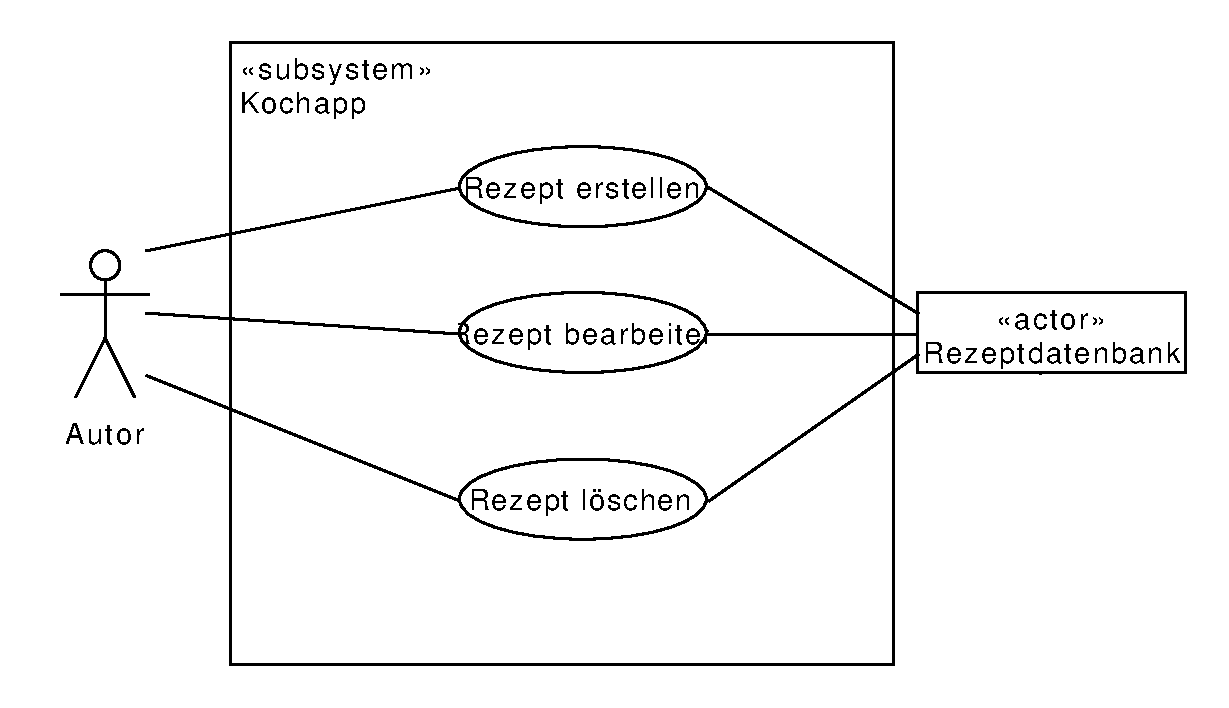
\includegraphics[width=0.8\textwidth]{grafiken/Anwendungsfalldiagramm_Rezeptverwaltung.pdf}
	\caption{Rezeptverwaltung von einem Autor}
		\end{center}
\end{figure}

\subsection{Interaktion mit öffentlichen Rezepten}
Im folgenden Diagramm wird die Interaktion mit öffentlichen Rezepten verdeutlicht. Ein Nutzer in der Rolle als \gls{Autor} publiziert sein privates Rezept, damit ist es als öffentliches Rezept verfügbar. Als \gls{Autor} kann er es auch wieder entfernen. 
Ein Nutzer in der Rolle als Rezeptsuchender kann es favorisieren, damit ist es bei ihm gespeichert. Er kann bewerten oder kommentieren. 

\begin{figure}[H]
\begin{center}
	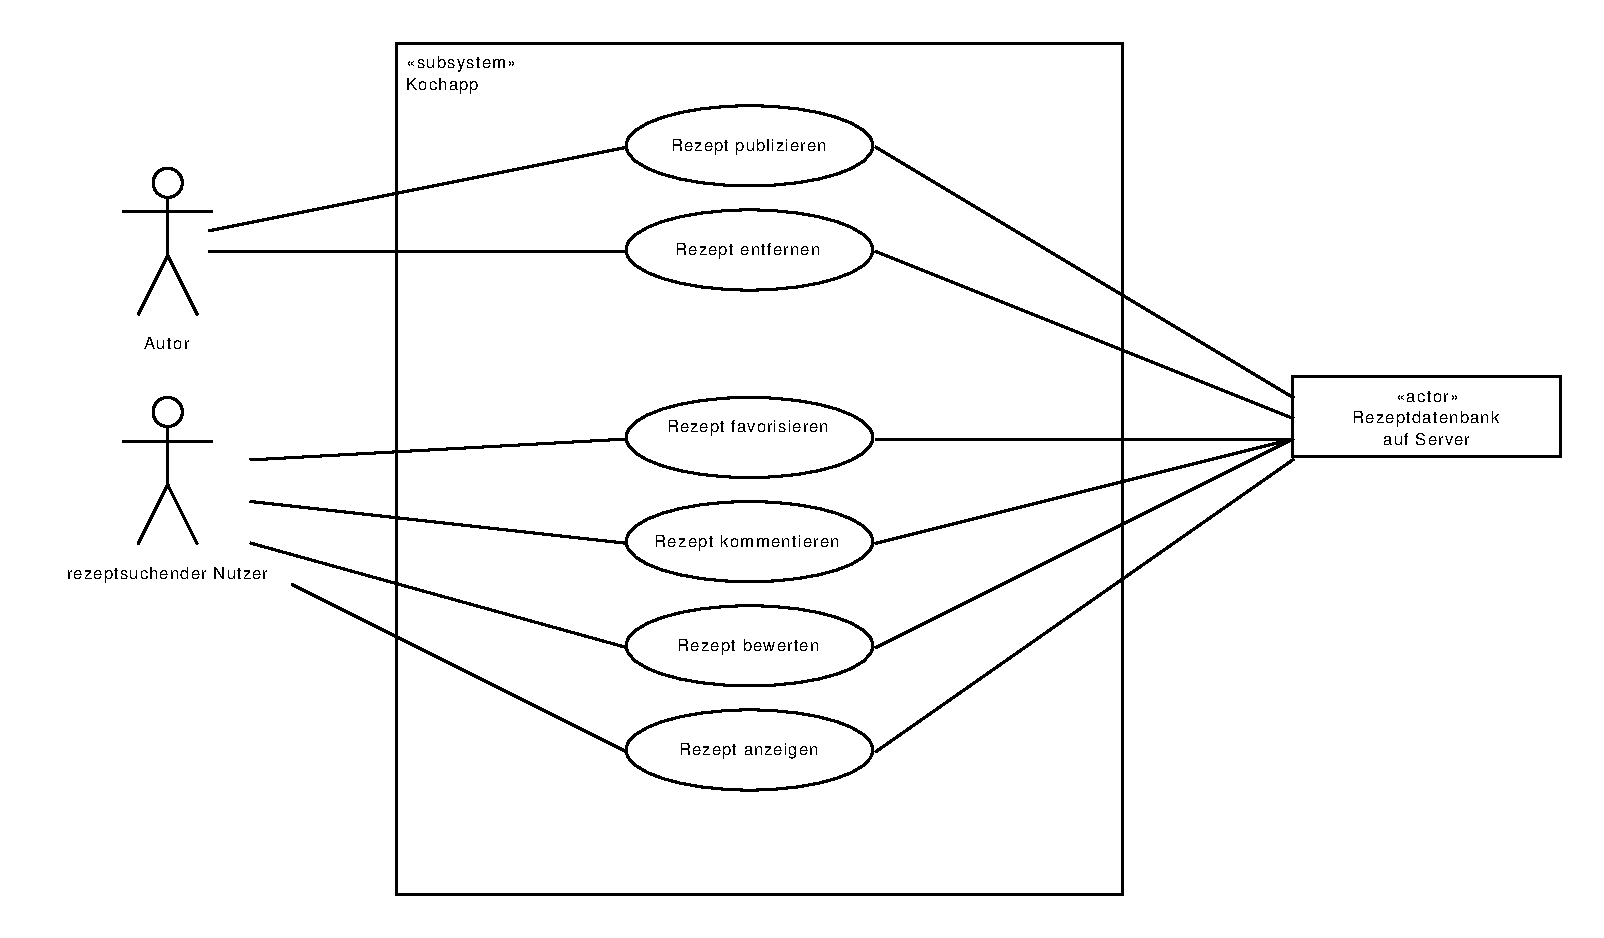
\includegraphics[width=1.0\textwidth]{grafiken/Anwendungsfalldiagramm_oeffentliche_Rezeptverwaltung.pdf}
	\caption{Aufgaben die ein Autor und ein rezeptsuchender Nutzer durchführen kann}
\end{center}
\end{figure}


\subsection{Benutzerverwaltung}
\begin{figure}[H]
\begin{center}
	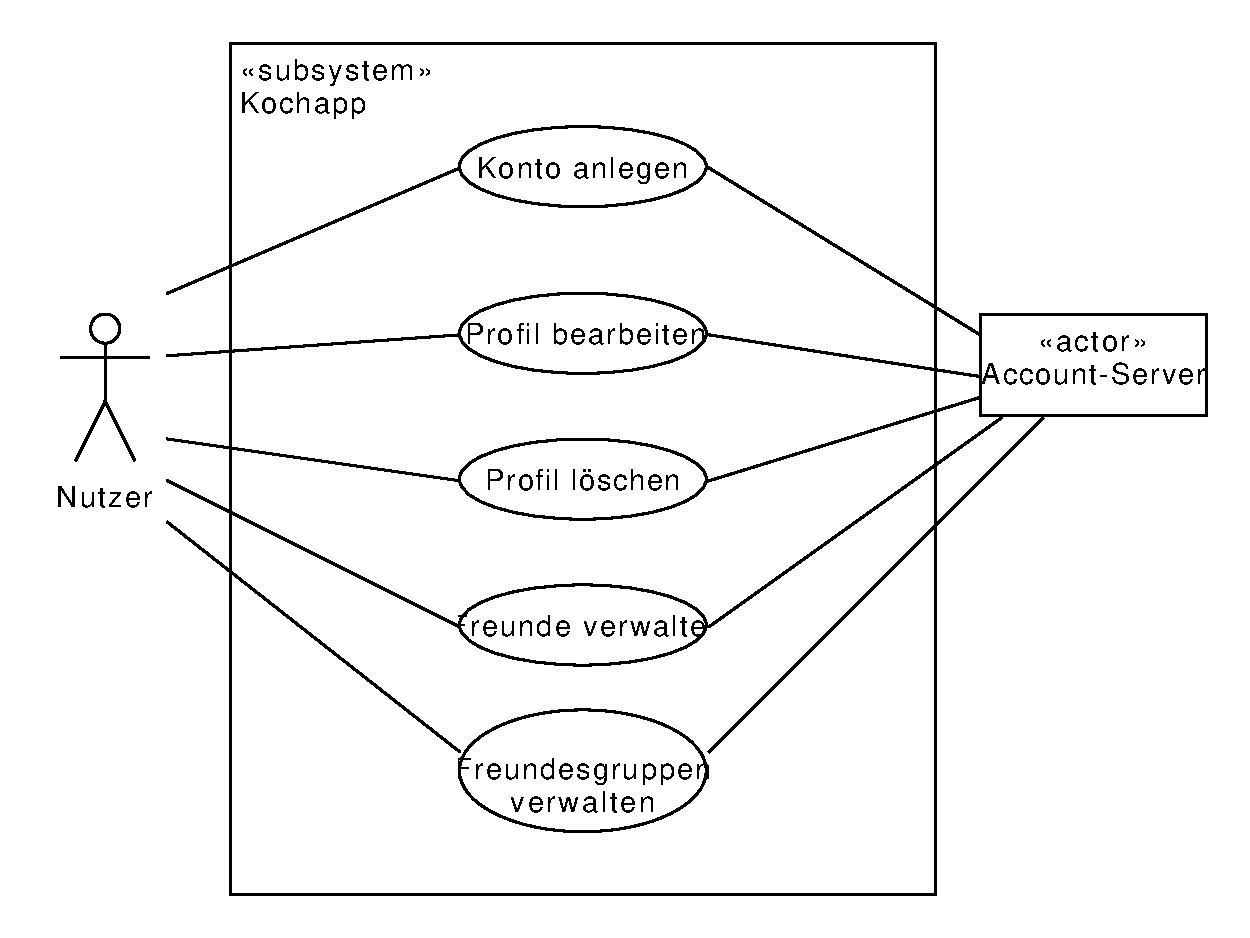
\includegraphics[width=0.8\textwidth]{grafiken/Anwendungsfalldiagramm_Benutzerverwaltung.pdf}
	\caption{Benutzerverwaltung eines Nutzers}
\end{center}
\end{figure}


%\subsection{Rezeptsuche}
%Todo suche noch in neues Diagramm oben eintragen. 
%\begin{center}
%	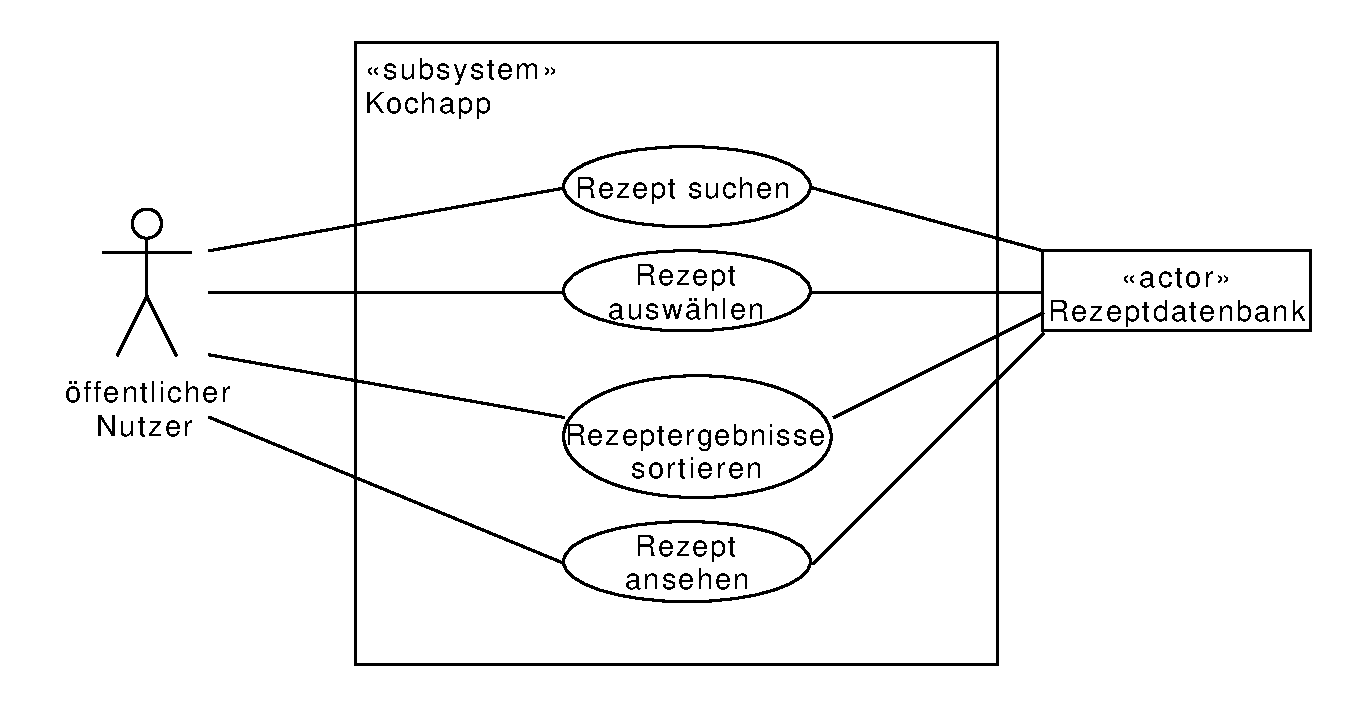
\includegraphics[width=0.8\textwidth]{grafiken/Anwendungsfalldiagramm_Rezeptsuchen.jpg}
%\end{center}




\section{Benutzeroberfläche}
Anbei sind exemplarisch Entwürfe einer möglichen Umsetzung der Benutzeroberfläche eingefügt. 

Die Benutzeroberfläche besteht aus verschiedenen Bereichen. 
Die Oberfläche hat einen Header (orange). 
Jede aufrufbare Seite der App hat ein Titel, der auf dem Header angezeigt wird.
Außerdem hat jede Seite verschiedene Elemente:
\begin{itemize}[nosep]
	\item Hintergrund (weiß)
	\item Textuelle Beschreibungen (schwarz)
	\item Eingabefelder (grau)
	\item Buttons (blau)
	\item Bilder (grün)
\end{itemize}

\subsection{Menü, Header und Suche}

\begin{figure}[H]
	\begin{minipage}[c]{.5\textwidth} 
		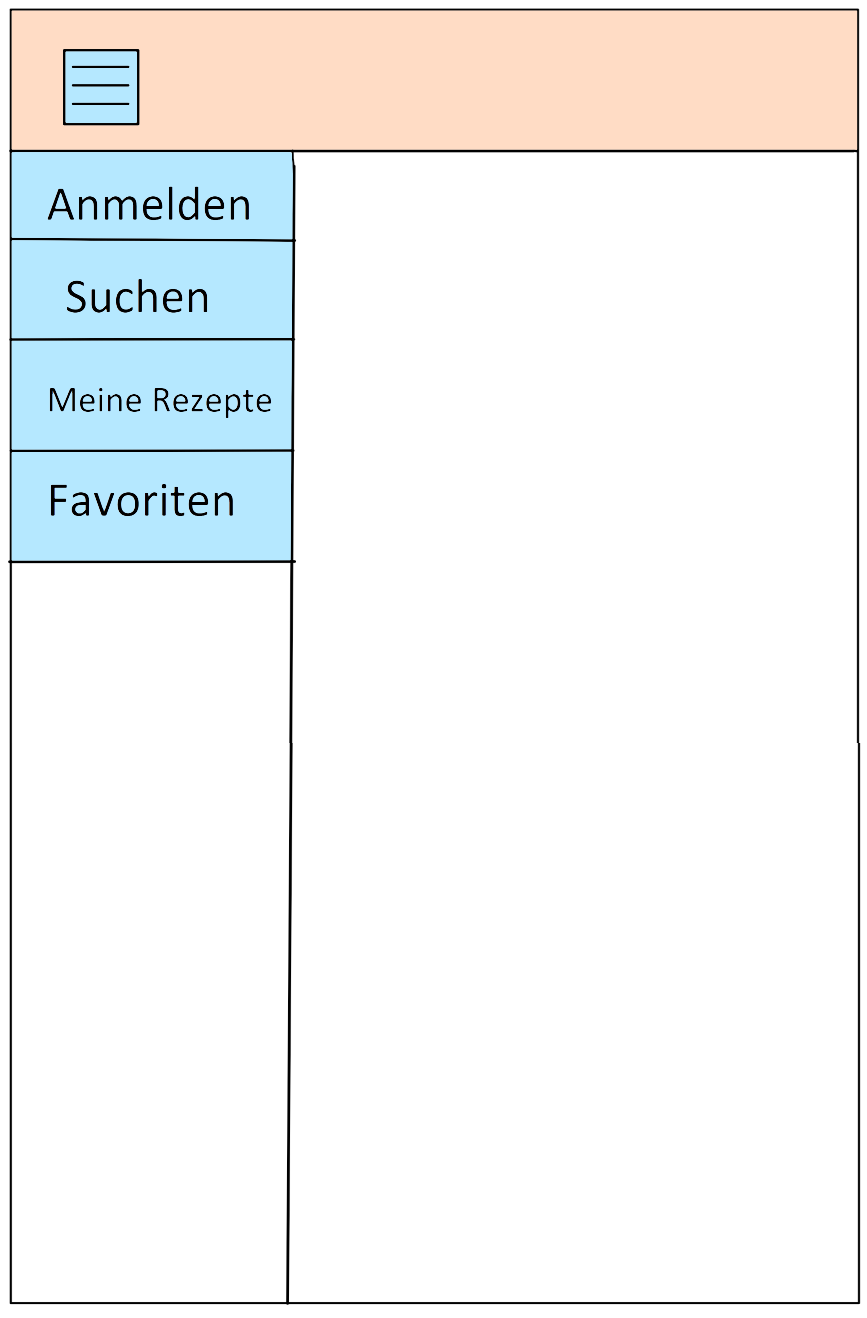
\includegraphics[width=\textwidth]{gui/seitenmenue.png}			
		\caption{Seitlich angezeigtes Menü der App}
		\label{menü}
	\end{minipage} \hspace{.7cm}
	\begin{minipage}[c]{.5\textwidth} 
			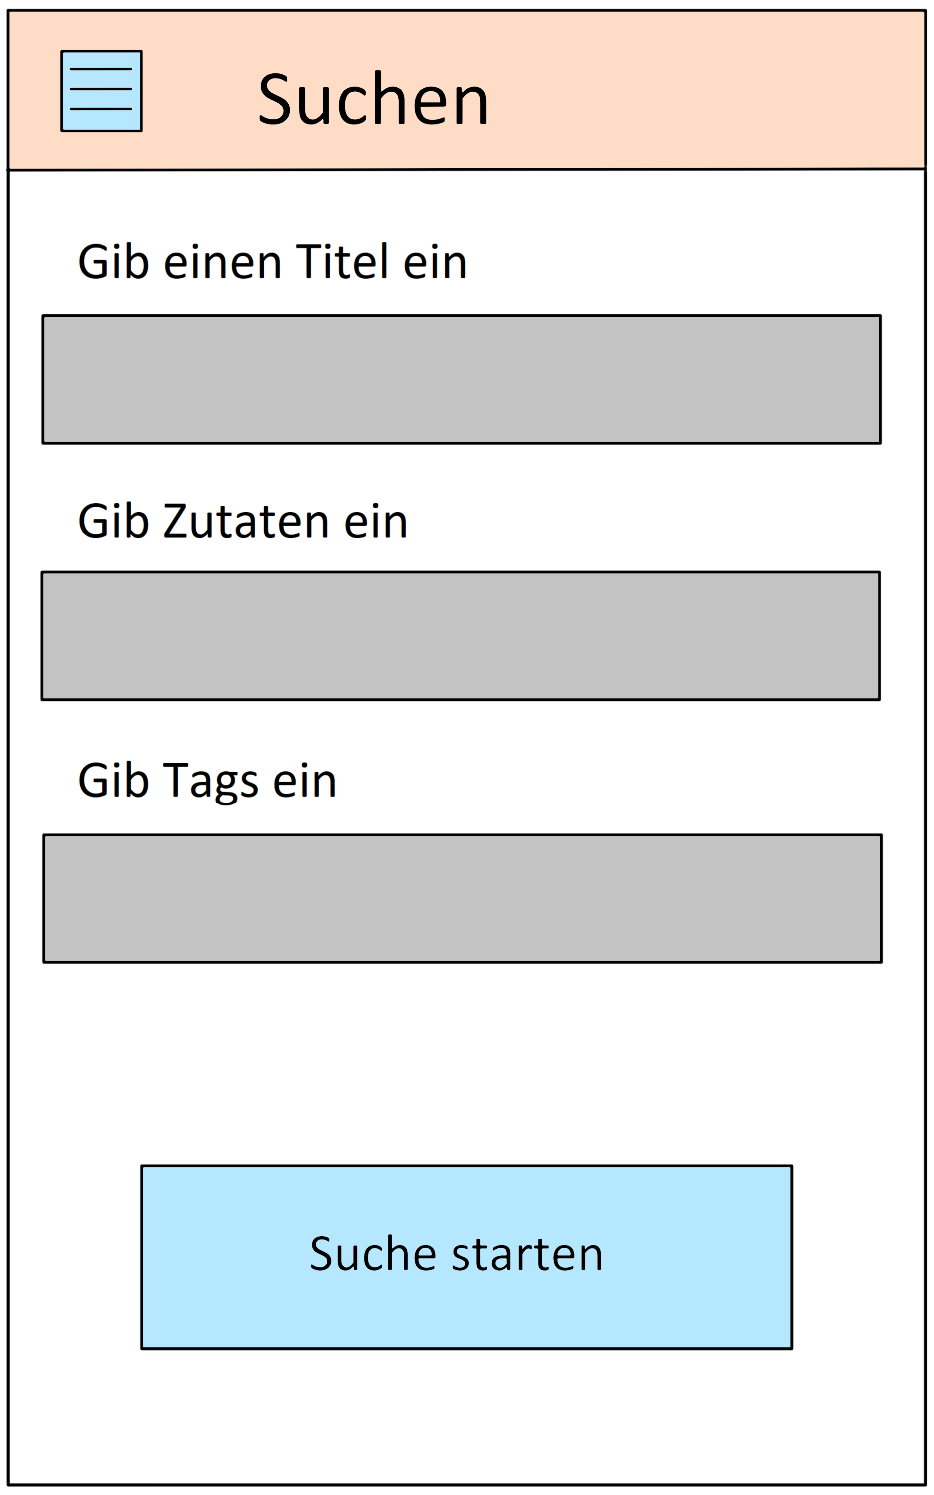
\includegraphics[width=\textwidth]{gui/suchen.png}				
		\caption{Suchfunktion mit Eingabefeldern und Buttons}
		\label{suche}
	\end{minipage}
\end{figure}


Das Menü in \ref{menü} zeigt die aufrufbaren Seiten der App. Es kann durch Klicken auf den Menübutton oben links auf dem Header ein- und ausgeblendet werden. Die Reiter im Menü sind Buttons, welche auf die jeweilig genannte Seite der App führen. Das Menü ist von jeder Seite der App aus erreichbar. Der Header ist ebenfalls immer über jeder Seite sichtbar. 

Skizze \ref{suche} zeigt die Suchfunktion. Nutzer können \gls{Suchfilter} in die Textfelder eingeben und die Suche dann starten. Die Suchseite ist auch die Startseite der App. Also die, die angezeigt wird, wenn ein Nutzer die App startet.


\subsection{Anmelden}

\begin{figure}[H]
	\begin{minipage}[c]{.5\textwidth} 
		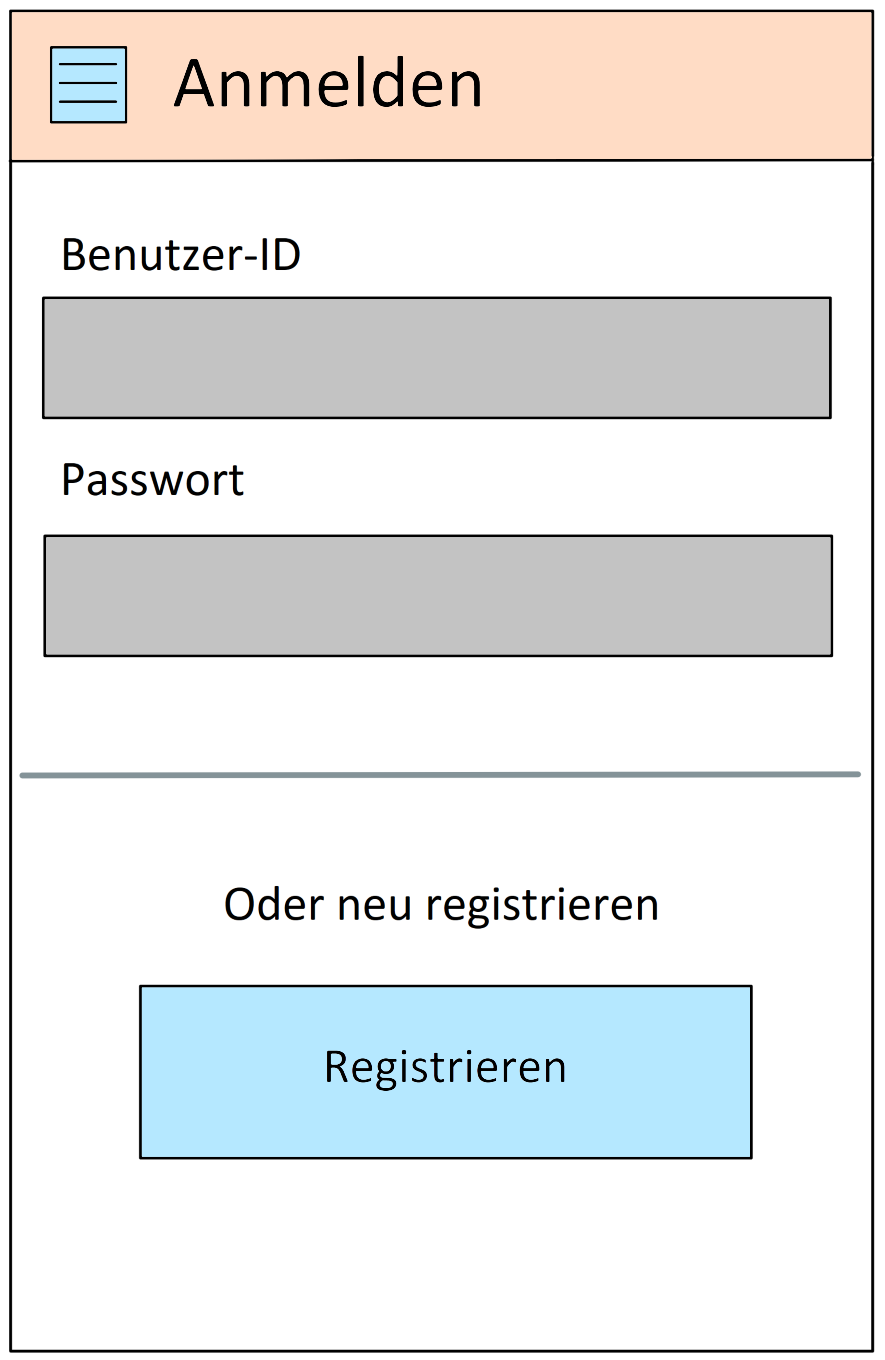
\includegraphics[width=\textwidth]{gui/anmelden.png}			
		\caption{Login-Seite}
		\label{anmelden}
	\end{minipage} \hspace{.7cm}
	\begin{minipage}[c]{.5\textwidth} 
			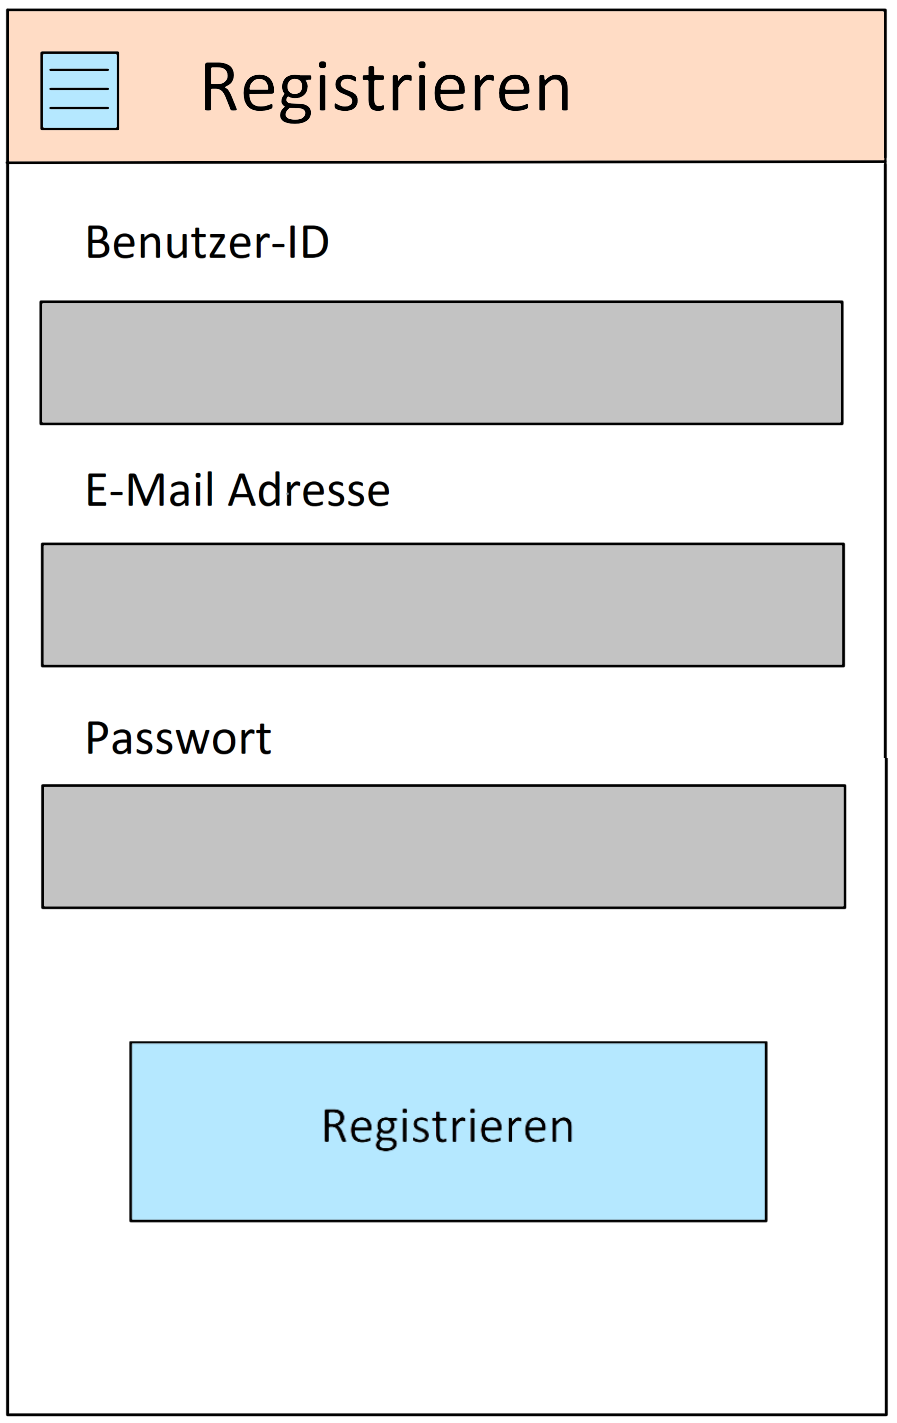
\includegraphics[width=\textwidth]{gui/registrieren.png}				
		\caption{Registrierung eines neuen Nutzers}
		\label{registrieren}
	\end{minipage}
\end{figure}

Die Login-Seite, die in \ref{anmelden} zu sehen ist, zeigt zwei Textfelder, in die der Nutzer die erforderlichen Anmeldeinformationen eintragen kann. Ist ein Nutzer noch nicht registriert, kommt er über den "`Registrieren"'-Button zur entsprechenden Seite.

Von der Login-Seite aus, kann ein Nutzer die Registrierungsseite erreichen, wie sie in \ref{registrieren} zu sehen ist. Hier kann er die nötigen Daten zur Registrierung angeben. Ist er fertig, drückt er auf den Button und wird in die Datenbank aufgenommen.



\subsection{Meine Rezepte}

\begin{figure}[H]
	\begin{minipage}[c]{.5\textwidth} 
		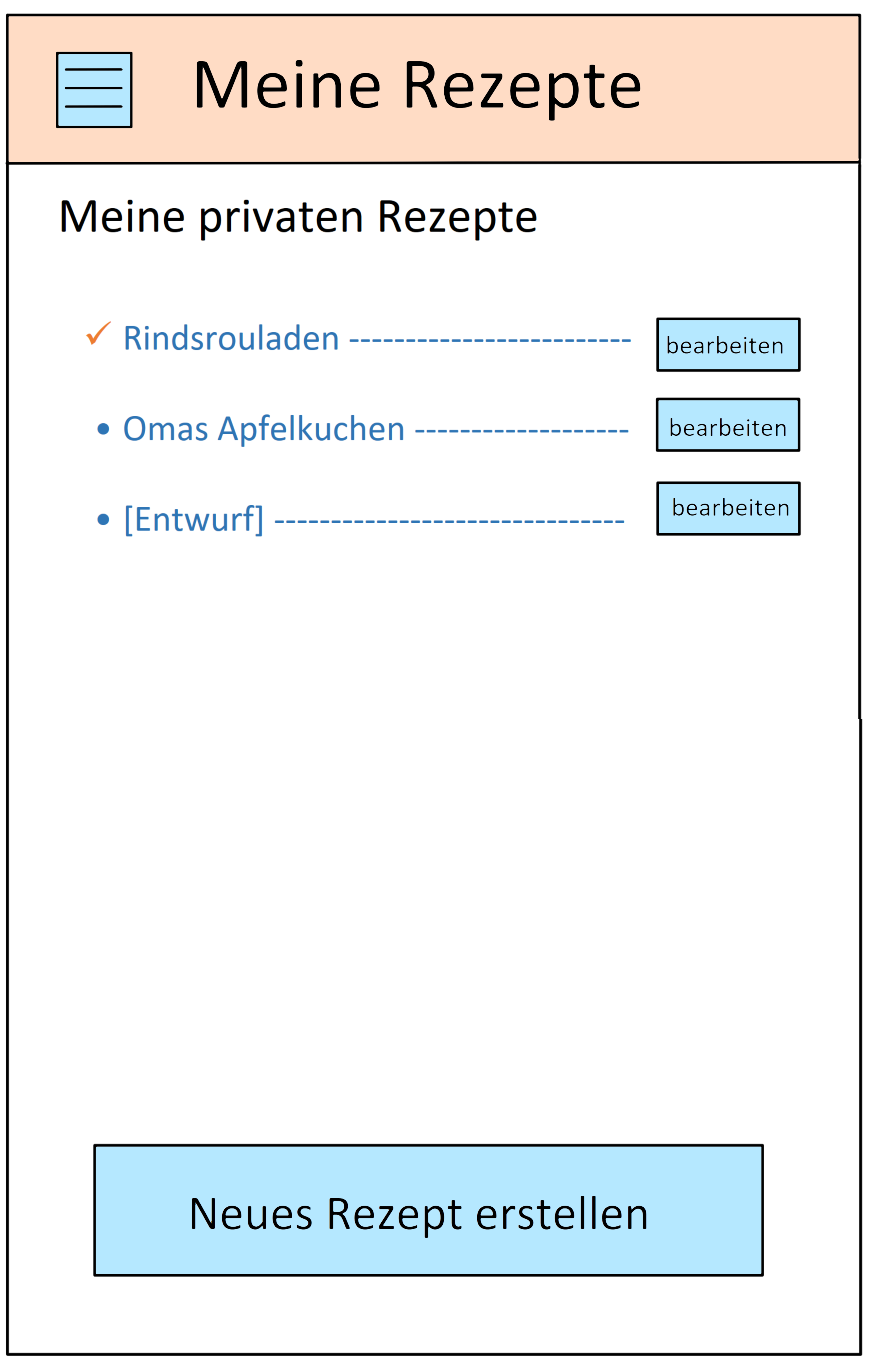
\includegraphics[width=\textwidth]{gui/meine_rezepte.png}	
		\caption{Abschnitt mit privaten und veröffentlichten Rezepten}
		\label{rezeptliste}
	\end{minipage} \hspace{.7cm}
	\begin{minipage}[c]{.5\textwidth} 
			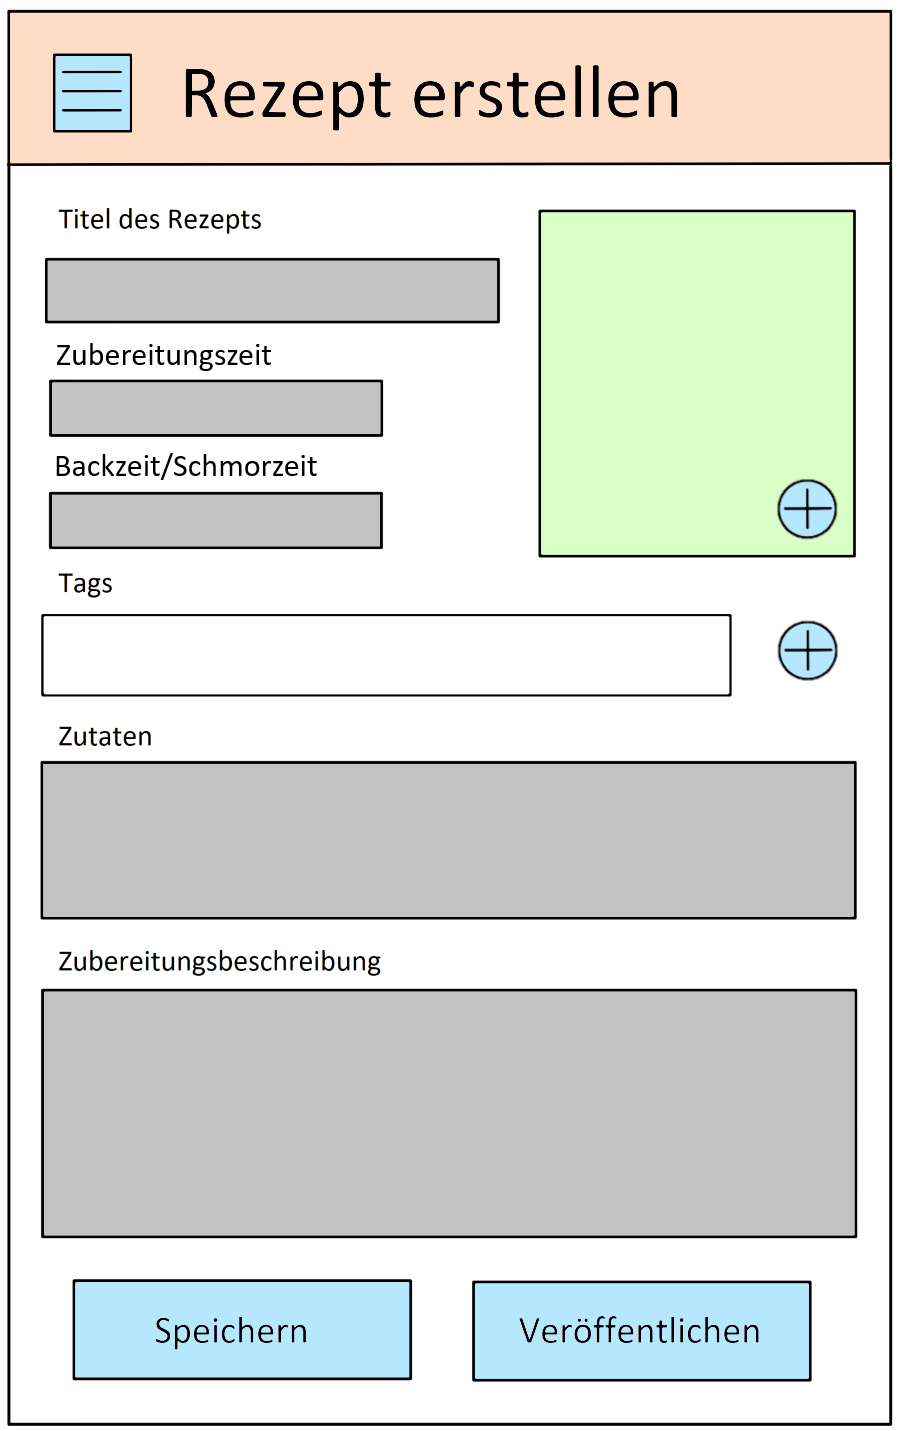
\includegraphics[width=\textwidth]{gui/rezept_erstellen.png}				
		\caption{Neues Rezept erstellen}
		\label{erstellen}
	\end{minipage}
\end{figure}


Abbildung \ref{rezeptliste} zeigt den Abschnitt "`Meine privaten Rezepte"'. Hier werden die Titel der Rezepte aus der \gls{Rezeptliste} eines Nutzers angezeigt. Rezepte, die noch keinen Titel haben, werden mit einem Platzhalter (hier: [Entwurf]) markiert. 
\Glspl{oRezept} haben dabei ein Häkchen, \glspl{pRezept} einen runden Punkt als führendes Icon. 
Über den "`bearbeiten"'-Button kann ein Rezept bearbeitet werden. 
Soll ein neues Rezept erstellt werden, kann der Nutzer das über den Button tun.

In \ref{erstellen} erstellt der Nutzer gerade ein neues Rezept. Er kann in die Textfelder entsprechende Informationen eintragen und über den runden Button im Bildfenster ein Bild hinzufügen. \glspl{Tag} kann er über den unteren runden Button neben dem "`\glspl{Tag}"'-Feld hinzufügen. Möchte er sein Rezept veröffentlichen, so klickt er auf "`Veröffentlichen"'. Hat der Nutzer das Rezept bereits veröffentlicht, zeigt dieser Button stattdessen "`Aktualisieren"' an. Der "`Speichern"'-Button gibt ihm die Möglichkeit, das Rezept manuell zu speichern. 




%
% % Automatisch generiertes Glossar (Latex zwei mal ausführen, um Glossar anzuzeigen)
%
%\glsaddall % das sorgt dafür, dass alles Glossareinträge gedruckt werden, nicht nur die verwendeten. Das sollte nicht nötig sein!
\printnoidxglossaries

\end{document}
